\chapter{Categorical Statements}
\label{chap:catstatements}
\markright{Chap. \ref{chap:catstatements}: Categorical Statements}
\setlength{\parindent}{1em}

% *********************************************
% * Quantified Categorical Statements
% **********************************************

\section{Quantified Categorical Statements}
\label{sec:qcatstatements}

Back in Chapter \ref{Chap:what_is_logic}, we saw that a statement was a unit of language that could be true or false. In this chapter and the next we are going to look at a particular kind of statement, called a quantified categorical statement, and begin to develop a formal theory of how to create arguments using these statements. This kind of logic is generally called ``categorical'' or ``Aristotelian'' logic, because it was originally invented by the great logician and philosopher Aristotle in the fourth century \textsc{bce}. This kind of logic dominated the European and Islamic worlds for 20 centuries afterward, and was expanded in all kinds of fascinating ways, some of which we will look at here.
 
%add a cross reference to the interesting historical sidebar for the Aristotelian tradition. 

Consider the following propositions:

\begin{enumerate}[label=(\alph*)]
\item \label{itm:dogs} All dogs are mammals.

\item \label{itm:physicists} Most physicists are male.

\item \label{itm:teachers} Few teachers are rock climbers.

\item \label{itm:no_dogs} No dogs are cats. 

\item \label{itm:americans} Some Americans are doctors. 

\item \label{itm:adults}Some adults are not logicians. 

\item \label{itm:canadians} Thirty percent of Canadians speak French.

\item \label{itm:chair}One chair is missing.

\end{enumerate}

\newglossaryentry{quantified categorical statement}
{
  %type=catstatements,
  name=quantified categorical statement,
  description={A statement that makes a claim about a certain quantity of the members of a class or group.}
}

These are all examples of quantified categorical statements. A  \textsc{\gls{quantified categorical statement}} \label{def:quantified_categorical_statement} is a statement that makes a claim about a certain quantity of the members of a class or group. (Sometimes we will just call these ``categorical statements'') Statement \ref{itm:dogs}, for example, is about the class of dogs and the class of mammals. These statements make no mention of any particular members of the categories or classes or types they are about. The propositions are also \textit{quantified} in that they state \textit{how many} of the things in one class are also members of the other. For instance, statement \ref{itm:physicists} talks about \textit{most} physicists, while statement \ref{itm:teachers} talks about \textit{few} teachers.  

\newglossaryentry{quantifier}
{
  %type=catstatements,
  name=quantifier,
  description={The part of a categorical sentence that specifies a portion of a class.}
}

\newglossaryentry{subject class}
{
  %type=catstatements,
  name=subject class,
  description={The first class named in a quantified categorical statement.}
}

\newglossaryentry{predicate class}
{
  %type=catsyllogisms,
  name=predicate class,
  description={The second class named in a quantified categorical statement.}
  }

\newglossaryentry{copula}
{
  name=copula,
  description={The form of the verb ``to be'' that links subject and predicate.}
}

Categorical statements can be broken down into four parts: the quantifier, the subject term, the predicate term, and the copula. The \textsc{\gls{quantifier}} \label{def:quantifier} is the part of a categorical sentence that specifies a portion of a class. It is the ``how many'' term. The quantifiers in the sentences above are all, most, few, no, some, thirty percent, and one. Notice that the ``no'' in sentence \ref{itm:no_dogs} counts as a quantifier, the same way zero counts as a number. The subject and predicate terms are the two classes the statement talks about. The \textsc{\gls{subject class}} \label{def:subject_class} is the first class mentioned in a quantified categorical statement, and the \textsc{\gls{predicate class}} \label{def:predicate_class} is the second. In sentence \ref{itm:americans}, for instance, the subject class is the class of Americans and the predicate class is the class of doctors.  The \textsc{\gls{copula}} \label{def:copula} is simply the form of the verb ``to be'' that links subject and predicate. Notice that the quantifier is always referring to the subject. The statement ``Thirty percent of Canadians speak French'' is saying something about a portion of Canadians, not about a portion of French speakers.

Sentence \ref{itm:canadians} is a little different than the others. In sentence \ref{itm:canadians} the subject is the class of Canadians and the predicate is the class of people who speak French. That's not quite the way it is written, however. There is no explicit copula, and instead of giving a noun phrase for the predicate term, like ``people who speak French,'' it has a verb phrase, ``speak French.'' If you are asked to identify the copula and predicate for a sentence like this, you should say that the copula is implicit and transform the verb phrase into a noun phrase. You would do something similar for sentence \ref{itm:chair}: the subject term is ``chair,'' and the predicate term is ``things that are missing.'' We will go into more detail about these issues in Section \ref{sec:transformation}.  


\begin{figure}
\begin{mdframed}[style=mytableclearbox]
\includegraphics*[width=\linewidth]{img/partsofacategoricalstatement}
\end{mdframed}
\caption{Parts of a quantified categorical statement.}
\label{fig:Partsofacategoricalstatement}
\end{figure}

In the previous chapter we noted that formal logic achieves content neutrality by replacing some or all of the ordinary words in a statement with symbols. For categorical logic, we are only going to be making one such substitution. Sometimes we will replace the classes referred to in a quantified categorical statement with capital letters that act as variables. Typically we will use the letter $S$ when referring to the class in the subject term and $P$ when referring to the predicate term, although sometimes more letters will be needed. Thus the sentence ``Some Americans are doctors,'' above, will sometimes become ``Some $S$ are $P$.'' The sentence ``No dogs are cats'' will sometimes become``No $S$ is $P$.''

 %%%%%%%%%%%%%% practice problems %%%%%%%%%%% 

\practiceproblems
\problempart For each of the following sentences identify the quantifier, the subject term, the predicate term, and the copula. Some of these are like the example ``Thirty percent of Canadians speak French'' where the copula is implicit and the predicate needs to be transformed into a noun phrase. 

\begin{longtabu}{p{.1\linewidth}p{.9\linewidth}}
\textbf{Example}: & Some dinosaurs had feathers\\
\textbf{Answer}: & Quantifier: Some \\
&Subject term: Dinosaurs \\
&Copula: Implicit \\
& Predicate term: Things with feathers \\
\end{longtabu}

\begin{exercises}
\item Some politicians are not members of tennis clubs.

\answer{
 Quantifier: Some \\
 Subject term: Politicians \\
 Copula: Are \\
 Predicate term: Things that are not members of tennis clubs \\ 
 }
\item All dogs go to heaven.

\answer{
 Quantifier:  All \\
 Subject term:  Dogs \\ 
 Copula:  Implicit \\
 Predicate term: Things that go to heaven \\
 }

\item Most things in the fridge are moldy.

\answer{
 Quantifier:  Most \\
 Subject term: Things in the fridge  \\
 Copula:  Are \\
 Predicate term: Things that are moldy  \\
}
\item Some birds do not fly.

\answer{
 Quantifier:  Some \\
 Subject term: Birds \\
 Copula: Implicit \\
 Predicate term: Things that do not fly. \\  
 }

\item Few people have seen Janet relaxed and happy.

\answer{
 Quantifier: Few  \\
 Subject term: People \\  
 Copula:  Implicit \\ 
 Predicate term:  People who have seen Janet relaxed and happy. \\
 }
\item No elephants are pocket-sized.

\answer{
 Quantifier: No \\
 Subject term:  Elephants \\
 Copula: Are  \\
 Predicate term: Things that are pocket sized. \\
}
\item Two thirds of Americans are obese or overweight.

\answer{
 Quantifier:  Two thirds \\
 Subject term:  Americans \\
 Copula:  Are\\
 Predicate term: People who are obese or overweight. \\
}
\item All applicants must submit to a background check. 

\answer{
 Quantifier:  All \\
 Subject term:  Applicants \\
 Copula:  Implicit \\
 Predicate term:  People who must submit to a background check. \\
 }
\item All handguns are weapons.

\answer{
 Quantifier:  All \\
 Subject term: Handguns  \\
 Copula:  Are\\
 Predicate term: Weapons  \\
 } 
\item One man stands alone against injustice.

\answer{
 Quantifier:  One \\
 Subject term:  Man \\
 Copula:  Implicit \\
 Predicate term:  People who stand alone against injustice. \\
 }
\end{exercises}



\noindent \problempart For each of the following sentences identify the quantifier, the subject term, the predicate term, and the copula. Some of these are like the example ``Thirty percent of Canadians speak French'' where the copula is implicit and the predicate needs to be transformed into a noun phrase. 


\begin{exercises}
\item No dog has been to Mars.

\answer{
 Quantifier:  No\\
 Subject term:  Dog\\
 Copula:  implicit\\
 Predicate term:  Things that have been to Mars \\
 }

\item All human beings are mortal.

\answer{
 Quantifier:  All\\
 Subject term:  Human beings\\
 Copula:  Are\\
 Predicate term:  Things that are mortal \\
 }

\item Some spears are six feet long.

\answer{
 Quantifier:  Some\\
 Subject term:  Spears \\
 Copula:  Are \\
 Predicate term:  Things that are six feet long \\
 }

\item Most dogs are friendly 

\answer{
 Quantifier:  Most\\
 Subject term:  Dogs\\
 Copula:  Are\\
 Predicate term:  Things that are friendly \\
 }

\item Eighty percent of Americans graduate from high school.

\answer{
 Quantifier:  Eighty percent\\
 Subject term:  Americans \\
 Copula:  Implicit\\
 Predicate term:   People who graduate from high school\\
 }

\item Few doctors are poor. 

\answer{
 Quantifier:  Few\\
 Subject term:  Doctors\\
 Copula:  Are\\
 Predicate term:   People who are poor\\
 }

\item All squids are cephalopods. 

\answer{
 Quantifier:  All\\
 Subject term:  Squids\\
 Copula:  Are \\
 Predicate term:   cephalopods\\
 }

\item No fish can sing.

\answer{
 Quantifier:  No\\
 Subject term:  Fish\\
 Copula:  Implicit\\
 Predicate term:  Things that can sing \\
 }

\item Some songs are sad.

\answer{
 Quantifier:  Some\\
 Subject term:  Songs\\
 Copula:  Are\\
 Predicate term:  Things that are sad \\
 }

\item Two dogs are playing in the backyard.

\answer{
 Quantifier:  Two \\
 Subject term:  Dogs \\
 Copula:  Are \\
 Predicate term:   Things that are playing in the backyard\\
 }

\end{exercises}


% **********************************
% * Quantity, Quality, and Distribution     *
% **********************************

\section{Quantity, Quality, Distribution, and Venn Diagrams}
\label{sec:QQDVD}
Ordinary English contains all kinds of quantifiers, including the counting numbers themselves. In this chapter and the next, however, we are only going to deal with two quantifiers: ``all,'' and ``some.'' We are restricting ourselves to the quantifiers ``all'' and ``some'' because they are the ones that can easily be combined to create valid arguments using the system of logic that was invented by Aristotle. We will deal with other quantifiers in chapter in the larger version of the text on induction. \label{ver_var} \nix{Chapter \ref{chap:induction}, on induction.} There we will talk about much more specific quantified statements, like ``Thirty percent of Canadians speak French,'' and do a little bit of work with modern statistical methods. 

\newglossaryentry{quantity}
{
name=quantity,
description={The portion of the subject class described by a categorical statement. Generally ``some'' or ``none.''}
}

\newglossaryentry{universal}
{
name=universal,
description={The quantity of a statement that uses the quantifier ``all.''}
}

\newglossaryentry{particular}
{
name=particular,
description={The quantity of a statement that uses the quantifier ``some.''}
}

The quantifier used in a statement is said to give the \textsc{\gls{quantity}} \label{def:Quantity} of the statement. Statements with the quantifier ``All'' are said to be ``\textsc{\gls{universal}}'' and those with the quantifier ``some'' are said to be ``\textsc{\gls{particular}}.''

Here ``some'' will just mean ``at least one.'' So, ``some people in the room are standing'' will be true even if there is only one person standing. Also, because ``some'' means ``at least one,'' it is compatible with ``all'' statements. If I say ``some people in the room are standing'' it might actually be that \textit{all} people in the room are standing, because if all people are standing, then at least one person is standing. This can sound a little weird, because in ordinary circumstances, you wouldn't bother to point out that something applies to some members of a class when, in fact, it applies to all of them. It sounds odd to say ``\textit{some} dogs are mammals,'' when in fact they \textit{all} are. Nevertheless, when ``some'' means ``at least one'' it is perfectly true that some dogs are mammals. 


\newglossaryentry{quality}
{
name=quality,
description={The status of a categorical statement as affirmative or negative.}
}

\newglossaryentry{negative}
{
name=negative,
description={The quality of a statement containing a ``not'' or ``no.''}
}

\newglossaryentry{affirmative}
{
name=affirmative,
description={The quality of a statement without a ``not'' or a ``no.''}
}



\newglossaryentry{statement mood}
{
name=statement mood,
description={The classification of a categorical statement based on its quantity and quality.}
}

\newglossaryentry{mood-A statement}
{
name=mood-A statement,
description={A quantified categorical statement of the form ``All $S$ are $P$.''}
}

\newglossaryentry{mood-E statement}
{
name=mood-E statement,
description={A quantified categorical statement of the form ``No $S$ are $P$.''}
}

\newglossaryentry{mood-I statement}
{
name=mood-I statement,
description={A quantified categorical statement of the form ``Some $S$ are $P$.''}
}

\newglossaryentry{mood-O statement}
{
name=mood-O statement,
description={A quantified categorical statement of the form ``Some $S$ are not $P$.''}
}



In addition to talking about the quantity of statements, we will talk about their \textsc{\gls{quality}}. \label{defQuality} The quality of a statement refers to whether the statement is negated. Statements that include the words ``no'' or ``not'' are \textsc{\gls{negative}}, and other statements are \textsc{\gls{affirmative}}. Combining quantity and quality gives us four basic types of quantified categorical statements, which we call the \textsc{\glspl{statement mood}} or just ``moods.'' The four moods are labeled with the letters A, E, I, and O. Statements that are universal and affirmative are \textsc{\glspl{mood-A statement}}. Statements that are universal and negative are \textsc{\glspl{mood-E statement}}. Particular and affirmative statements are \textsc{\glspl{mood-I statement}}, and particular and negative statements are \textsc{\glspl{mood-O statement}}. (See Table \ref{tab:moods}.)


Aristotle didn't actually use those letters to name the kinds of categorical propositions. His later followers writing in Latin came up with the idea. They remembered the labels because the ``A'' and the ``I'' were in the Latin word ``\textbf{a}ff\textbf{i}rmo,'' (``I affirm'') and the ``E'' and the ``O'' were in the Latin word ``n\textbf{e}g\textbf{o}'' (``I deny''). 

\begin{table}[t]
\begin{mdframed}[style=mytablebox]
\begin{tabu}{p{.1\linewidth}p{.3\linewidth}p{.3\linewidth}}
  \underline{Mood}& \underline{Form} & \underline{Example} \\ 
A & All $S$ are $P$ & All dogs are mammals. \\
E & No S are $P$ & No dogs are reptiles. \\
I & Some $S$ are $P$ & Some birds can fly. \\
O & Some $S$ are not $P$ & Some birds cannot fly.\\
\end{tabu}
\end{mdframed}
\caption{The four moods of a categorical statement} \label{tab:moods}
\end{table}

\newglossaryentry{distribution}
{
name=distribution,
description={A property of the terms of a categorical statement that is present when the statement makes a claim about the whole term.}
}

The \textsc{\gls{distribution}} of a categorical statement refers to how the statement describes its subject and predicate class. A term in a sentence is said to be distributed \label{def:Distribution} if a claim is being made about the whole class. In the sentence ``All dogs are mammals,'' the subject class, dogs, is distributed, because the quantifier ``All'' refers to the subject. The sentence is asserting that every dog out there is a mammal. On the other hand, the predicate class, mammals, is not distributed, because the sentence isn't making a claim about all the mammals. We can infer that at least some of them are dogs, but we can't infer that all of them are dogs. So in mood-A statements, only the subject is distributed. 

On the other hand, in an I sentence like ``Some birds can fly'' the subject is not distributed. The quantifier ``some'' refers to the subject, and indicates that we are not saying something about all of that subject. We also aren't saying anything about all flying things, either. So in mood-I statements, neither subject nor predicate is distributed. 

Even though the quantifier always refers to the subject, the predicate class can be distributed as well. This happens when the statement is negative. The sentence ``No dogs are reptiles'' is making a claim about all dogs: they are all not reptiles. It is also making a claim about all reptiles: they are all not dogs. So mood-E statements distribute both subject and predicate. Finally, negative particular statements (mood-O) have only the predicate class distributed. The statement ``some birds cannot fly'' does not say anything about all birds. It does, however say something about all flying things: the class of all flying things excludes some birds. 

The quantity, quality, and distribution of the four forms of a categorical statement are given in Table \ref{tab:quantity}. The general rule to remember here is that universal statements distribute the subject, and negative statements distribute the predicate. 


\begin{table}[b]
\begin{mdframed}[style=mytablebox]
\begin{tabu}{p{.1\linewidth}p{.2\linewidth}p{.15\linewidth}p{.15\linewidth}p{.4\linewidth}}
 \underline{Mood} & \underline{Form} &  \underline{Quantity} & \underline{Quality} & \underline{Terms Distributed} \\ 
A & All $S$ are $P$ & Universal &  Affirmative & S\\
E & No $S$ are $P$ & Universal & Negative & S and P\\
I & Some $S$ are $P$ & Particular & Affirmative & None\\
O &Some $S$ are not $P$ & Particular &Negative & P \\
\end{tabu}
\end{mdframed}
\caption{Quantity, quality, and distribution.}\label{tab:quantity}
\end{table}

\newglossaryentry{Venn diagram}
{
name=Venn diagram,
description={A diagram that represents categorical statements using circles that stand for classes.}
}


In 1880 English logician John Venn published two essays on the use of diagrams with circles to represent categorical propositions (Venn \citeyear{Venn1880a}, \citeyear{Venn1880b}). Venn noted that the best use of such diagrams so far had come from the brilliant Swiss mathematician Leonhard Euler, but they still had many problems, which Venn felt could be solved by bringing in some ideas about logic from his fellow English logician George Boole. Although Venn only claimed to be building on the long logical tradition he traced, since his time these kinds of circle diagrams have been known as \textsc{\glspl{Venn diagram}}.

In this section we are going to learn to use Venn diagrams to represent our four basic types of categorical statement. Later in this chapter, we will find them useful in evaluating arguments. Let us start with a statement in mood A: ``All $S$ are $P$.'' We are going to use one circle to represent $S$ and another to represent $P$. There are a couple of different ways we could draw the circles if we wanted to represent ``All $S$ are $P$.'' One option would be to draw the circle for $S$ entirely inside the circle for $P$, as in Figure \ref{fig:euler_circles}

\begin{figure}
\begin{mdframed}[style=mytablehalfbox]
\begin{center}
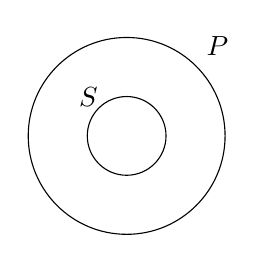
\begin{tikzpicture}
\def\firstcircle{(0,0) circle (.5 cm)}
\def\secondcircle{(0:0) circle (1.25 cm)}
\draw \firstcircle node[outer sep=.25cm, above left] (s) {$S$};
\draw \secondcircle node[outer sep=.9cm, above right] (p) {$P$};
\end{tikzpicture}
\end{center}
\end{mdframed}
\caption{Euler Circles} \label{fig:euler_circles}
\end{figure}

\begin{figure}
\begin{mdframed}[style=mytableclearbox, userdefinedwidth=.3\textwidth]
\begin{center}
\includegraphics*{img/OriginalVenn}
\end{center}
\end{mdframed}
\caption{Venn's original \\ diagram for an mood-A statement \\(Venn \citeyear{Venn1880a}).}
\end{figure}


It is clear from Figure \ref{fig:euler_circles} that all $S$ are in fact $P$. And outside of college logic classes, you may have seen people use a diagram like this to represent a situation where one group is a subclass of another. You may have even seen people call concentric circles like this a Venn diagram. But Venn did not think we should put one circle entirely inside the other if we just want to represent ``All $S$ is $P$.'' Technically speaking Figure \ref{fig:euler_circles} shows Euler circles.

Venn pointed out that the circles in Figure \ref{fig:euler_circles} don't just say that ``All $S$ are $P$.'' They also says that ``All $P$ are $S$'' is false. But we don't necessarily know that if we have only asserted ``All $S$ are $P$.'' The statement ``All $S$ are $P$'' leaves it open whether the $S$ circle should be smaller than or the same size as the $P$ circle.

Venn suggested that to represent just the content of a single proposition, we should always begin by drawing partially overlapping circles. This means that we always have spaces available to represent the four possible ways the terms can combine: 

\begin{center}
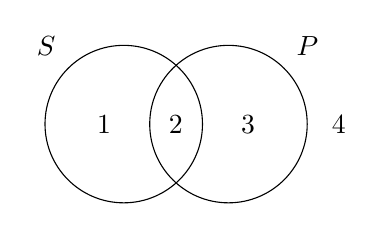
\begin{tikzpicture}
\def\firstcircle{(0,0) circle (1cm)}
\def\secondcircle{(0:1.33cm) circle (1cm)}
\draw \firstcircle node[outer sep=.75cm, above left] (s) {$S$} 
	node [xshift=-.25cm] (1) {1}
	node [xshift=.66cm] (2){2};
\draw \secondcircle node[outer sep=.75cm, above right] (p) {$P$}
	node [xshift=.25cm] (3) {3}
	node [xshift=1.4cm] (4){4};
\end{tikzpicture}
\label{fig:two_circle_venn}
\end{center}

Area 1 represents things that are $S$ but not $P$; area 2, things that are $S$ and $P$; area 3, things that are just $P$; and area 4 represents things that are neither $S$ nor $P$. We can then mark up these areas to indicate whether something is there or could be there. We shade a region of the diagram to represent the claim that nothing can exist in that region. For instance, if we say ``All $S$ are $P$,'' we are asserting that nothing can exist that is in the $S$ circle unless it is also in the $P$ circle. So we shade out the part of the $S$ circle that doesn't overlap with $P$. 

\begin{center}
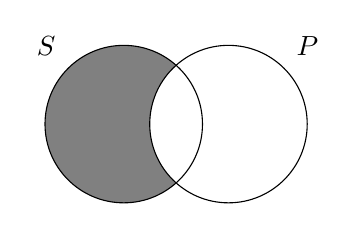
\begin{tikzpicture}
\def\firstcircle{(0,0) circle (1cm)}
\def\secondcircle{(0:1.33cm) circle (1cm)}
     \begin{scope}[shift={(4cm,0cm)}]
        \begin{scope}[even odd rule]% first circle without the second
            \clip \secondcircle (-1,-1) rectangle (1,1);
        \fill[gray] \firstcircle;
        \end{scope}
        \draw \firstcircle node[outer sep=.75cm, above left] (s) {$S$};
        \draw \secondcircle node[outer sep=.75cm, above right] (p) {$P$};
    \end{scope} 
\end{tikzpicture}
\end{center}


If we want to say that something does exist in a region, we put an ``x'' in it. This is the diagram for ``Some $S$ are $P$'': 

\begin{center}
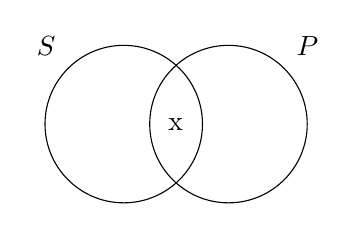
\begin{tikzpicture}
\def\firstcircle{(0,0) circle (1cm)}
\def\secondcircle{(0:1.33cm) circle (1cm)}
\draw \firstcircle node[outer sep=.75cm, above left] (s) {$S$};
\node[outer sep=.45cm, right] (x) {x};
\draw \secondcircle node[outer sep=.75cm, above right] (p) {$P$};
\end{tikzpicture}
\end{center}

If a region of a Venn diagram is blank, if it is neither shaded nor has an x in it, it could go either way. Maybe such things exist, maybe they do not.

The Venn diagrams for all four basic forms of categorical statements are in Figure \ref{fig:fourvenns}. Notice that when we draw diagrams for the two universal forms, A and E, we do not draw any x's. For these forms we are only ruling out possibilities, not asserting that things actually exist. This is part of what Venn learned from Boole, and we will see its importance in Section \ref{sec:ExistentialImport}. 

Finally, notice that so far, we have only been talking about categorical statements involving the variables $S$ and $P$. Sometimes, though, we will want to represent statements in regular English. To do this, we will include a dictionary saying what the variables $S$ and $P$ represent in this case. For instance, this is the diagram for ``No dogs are reptiles.''

\begin{figure}[H]
\begin{center}
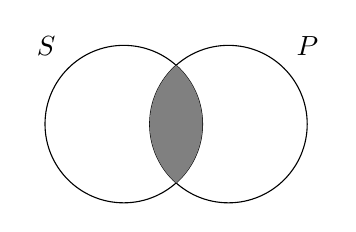
\begin{tikzpicture}
\def\firstcircle{(0,0) circle (1cm)}
\def\secondcircle{(0:1.33cm) circle (1cm)}
\draw \firstcircle node[outer sep=.75cm, above left] (s) {$S$};
\draw \secondcircle node[outer sep=.75cm, above right] (p) {$P$};
    \begin{scope}
      \clip \firstcircle;
      \fill[gray] \secondcircle;
    \end{scope}
\end{tikzpicture}
\captionsetup{singlelinecheck=on}
\caption*{$S$: Dogs \\ $P$: Reptiles}
\end{center}
\end{figure}



\begin{figure}
\begin{mdframed}[style=mytablebox]
\begin{tabu}{X[1,c,m]X[1,c,m]}

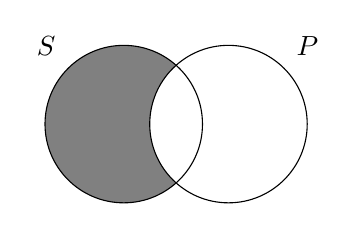
\begin{tikzpicture}
\def\firstcircle{(0,0) circle (1cm)} 
\def\secondcircle{(0:1.33cm) circle (1cm)}
     \begin{scope}[shift={(4cm,0cm)}]
        \begin{scope}[even odd rule]% first circle without the second
            \clip \secondcircle (-1,-1) rectangle (1,1);
        \fill[gray] \firstcircle;
        \end{scope}
        \draw \firstcircle node[outer sep=.75cm, above left] (s) {$S$};
        \draw \secondcircle node[outer sep=.75cm, above right] (p) {$P$};
    \end{scope} 
\end{tikzpicture}

&


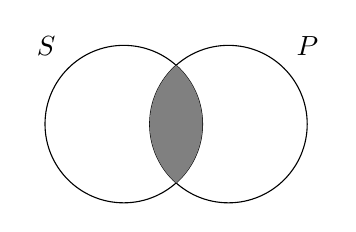
\begin{tikzpicture}
\def\firstcircle{(0,0) circle (1cm)}
\def\secondcircle{(0:1.33cm) circle (1cm)}
\draw \firstcircle node[outer sep=.75cm, above left] (s) {$S$};
\draw \secondcircle node[outer sep=.75cm, above right] (p) {$P$};
    \begin{scope}
      \clip \firstcircle;
      \fill[gray] \secondcircle;
    \end{scope}
\end{tikzpicture}


\\

\textbf{A}: All $S$ are $P$

&

\textbf{E}: No $S$ are $P$


\\
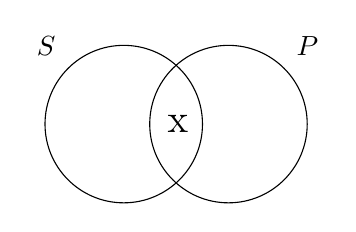
\begin{tikzpicture}
\def\firstcircle{(0,0) circle (1cm)}
\def\secondcircle{(0:1.33cm) circle (1cm)}
\draw \firstcircle node[outer sep=.75cm, above left] (s) {$S$};
\node[outer sep=.44cm, right] (x) {\Large{x}};
\draw \secondcircle node[outer sep=.75cm, above right] (p) {$P$};
\end{tikzpicture}

&

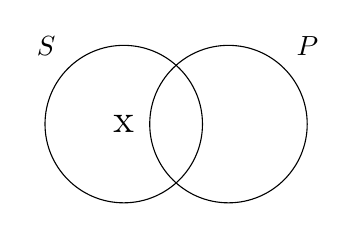
\begin{tikzpicture}
\def\firstcircle{(0,0) circle (1cm)}
\def\secondcircle{(0:1.33cm) circle (1cm)}
\draw \firstcircle node[outer sep=.75cm, above left] (s) {$S$};
\node[outer sep=.3cm] (x) {\Large{x}};
\draw \secondcircle node[outer sep=.75cm, above right] (p) {$P$};
\end{tikzpicture}

\\

\textbf{I}: Some $S$ are $P$
&
\textbf{O}: Some $S$ are not $P$

\end{tabu}
\end{mdframed}
\caption{Venn Diagrams for the Four Basic Forms of a Categorical Statement}
\label{fig:fourvenns}
\end{figure}

%%%%%%%%%%%%%%% Practice problems %%%%%%%%%%

\practiceproblems

\problempart Identify each of the following sentences as A, E, I, or O; state its quantity and quality; and state which terms are distributed. Then draw the Venn Diagram for each.

\begin{longtabu}{p{.1\linewidth}p{.9\linewidth}}
\textbf{Example}: & Some dinosaurs are not herbivores \\
\textbf{Answer}: & Form: O\\
&Quantity: particular \\
&Quality: negative \\
&
%\vspace{.25em}
\noindent 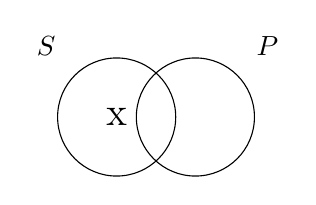
\begin{tikzpicture}
\def\firstcircle{(0,0) circle (.75cm)}
\def\secondcircle{(0:1cm) circle (.75cm)}
\draw \firstcircle node[outer sep=.66cm, above left] (s) {$S$};
\node[outer sep=.3cm] (x) {\Large{x}};
\draw \secondcircle node[outer sep=.66cm, above right] (p) {$P$};
\end{tikzpicture}\\
& $S$: Dinosaurs \\
& $P$: Herbivores
\end{longtabu}

\begin{exercises}

\item All gerbils are rodents.

\answer{
Form: A\\
Quantity: Universal \\
Quality: Affirmative\\

\vspace{.25em}

\noindent 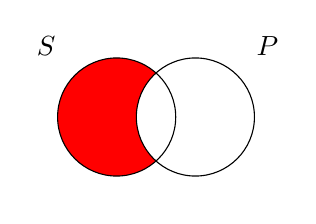
\begin{tikzpicture}
\def\firstcircle{(0,0) circle (.75cm)}
\def\secondcircle{(0:1cm) circle (.75cm)}
       \begin{scope}[even odd rule]% first circle without the second
            \clip \secondcircle (-1,-1) rectangle (1,1);
        \fill[red] \firstcircle;
        \end{scope}
 \draw \firstcircle node[outer sep=.66cm, above left] (s) {$S$};
%\node[outer sep=.3cm] (x) {\Large{x}};
\draw \secondcircle node[outer sep=.66cm, above right] (p) {$P$};
\end{tikzpicture}\\
$S$: Gerbils\\
$P$: Rodents
}

\item Some planets do not have life.

\answer{
Form: O\\
Quantity: Particular \\
Quality: Negative \\

\vspace{.25em}
\noindent 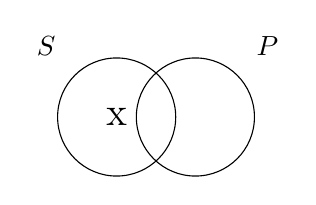
\begin{tikzpicture}
\def\firstcircle{(0,0) circle (.75cm)}
\def\secondcircle{(0:1cm) circle (.75cm)}
\draw \firstcircle node[outer sep=.66cm, above left] (s) {$S$};
\node[outer sep=.3cm] (x) {\Large{x}};
\draw \secondcircle node[outer sep=.66cm, above right] (p) {$P$};
\end{tikzpicture}\\
 $S$: Planets\\
 $P$: Things that have life
}

\item Some manatees are not rappers.

\answer{
Form: O\\
Quantity: Particular \\
Quality: Negative \\

\vspace{.25em}
\noindent 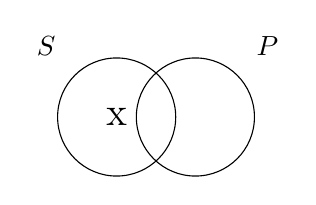
\begin{tikzpicture}
\def\firstcircle{(0,0) circle (.75cm)}
\def\secondcircle{(0:1cm) circle (.75cm)}
\draw \firstcircle node[outer sep=.66cm, above left] (s) {$S$};
\node[outer sep=.3cm] (x) {\Large{x}};
\draw \secondcircle node[outer sep=.66cm, above right] (p) {$P$};
\end{tikzpicture}\\
 $S$: Manatees\\
 $P$: Rappers
}


\item All rooms have televisions.

\answer{
Form: A\\
Quantity: Universal \\
Quality: Affirmative\\

\vspace{.25em}

\noindent 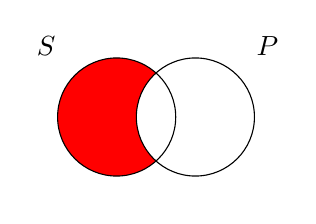
\begin{tikzpicture}
\def\firstcircle{(0,0) circle (.75cm)}
\def\secondcircle{(0:1cm) circle (.75cm)}
       \begin{scope}[even odd rule]% first circle without the second
            \clip \secondcircle (-1,-1) rectangle (1,1);
        \fill[red] \firstcircle;
        \end{scope}
 \draw \firstcircle node[outer sep=.66cm, above left] (s) {$S$};
%\node[outer sep=.3cm] (x) {\Large{x}};
\draw \secondcircle node[outer sep=.66cm, above right] (p) {$P$};
\end{tikzpicture}\\
$S$: Rooms\\
$P$: Things that have televisions
}


\item All stores are closed.

\answer{
Form: A\\
Quantity: Universal \\
Quality: Affirmative\\

\vspace{.25em}

\noindent 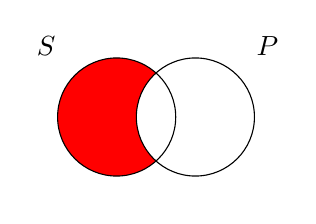
\begin{tikzpicture}
\def\firstcircle{(0,0) circle (.75cm)}
\def\secondcircle{(0:1cm) circle (.75cm)}
       \begin{scope}[even odd rule]% first circle without the second
            \clip \secondcircle (-1,-1) rectangle (1,1);
        \fill[red] \firstcircle;
        \end{scope}
 \draw \firstcircle node[outer sep=.66cm, above left] (s) {$S$};
%\node[outer sep=.3cm] (x) {\Large{x}};
\draw \secondcircle node[outer sep=.66cm, above right] (p) {$P$};
\end{tikzpicture}\\
$S$: Stores\\
$P$: Things that are closed
}


\item Some dancers are graceful. 

\answer{
Form: I\\
Quantity: Particular \\
Quality: Affirmative\\

\vspace{.25em}

\noindent 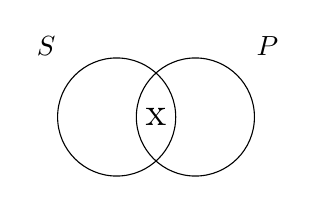
\begin{tikzpicture}
\def\firstcircle{(0,0) circle (.75cm)}
\def\secondcircle{(0:1cm) circle (.75cm)}
%       \begin{scope}[even odd rule]% first circle without the second
%            \clip \secondcircle (-1,-1) rectangle (1,1);
%        \fill[red] \firstcircle;
%        \end{scope}
 \draw \firstcircle node[outer sep=.66cm, above left] (s) {$S$};
%\node[outer sep=.3cm] (x) {\Large{x}};
\node[outer sep=.3cm, xshift=.5cm] (x) {\Large{x}};
\draw \secondcircle node[outer sep=.66cm, above right] (p) {$P$};
\end{tikzpicture}\\
$S$: Dancers\\
$P$: Things that are graceful
}


\item No extraterrestrials are in Cleveland. 

\answer{
Form: E\\
Quantity: Universal \\
Quality: Negative\\

\vspace{.25em}

\noindent 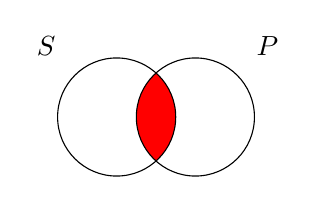
\begin{tikzpicture}
\def\firstcircle{(0,0) circle (.75cm)}
\def\secondcircle{(0:1cm) circle (.75cm)}
%       \begin{scope}[even odd rule]% first circle without the second
%            \clip \secondcircle (-1,-1) rectangle (1,1);
%        \fill[red] \firstcircle;
%        \end{scope}
    \begin{scope}
      \clip \firstcircle;
      \fill[red] \secondcircle;
    \end{scope}
\draw \firstcircle node[outer sep=.66cm, above left] (s) {$S$};
%\node[outer sep=.3cm] (x) {\Large{x}};
%\node[outer sep=.3cm, xshift=.5cm] (x) {\Large{x}};
\draw \secondcircle node[outer sep=.66cm, above right] (p) {$P$};
\end{tikzpicture}\\
$S$: Extraterrestrial\\
$P$: Things in Cleveland
}

\item Some crates are empty.

\answer{
Form: I\\
Quantity: Particular \\
Quality: Affirmative\\

\vspace{.25em}

\noindent 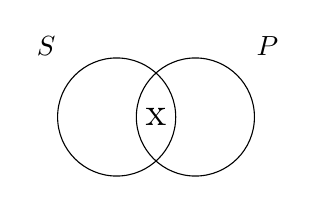
\begin{tikzpicture}
\def\firstcircle{(0,0) circle (.75cm)}
\def\secondcircle{(0:1cm) circle (.75cm)}
%       \begin{scope}[even odd rule]% first circle without the second
%            \clip \secondcircle (-1,-1) rectangle (1,1);
%        \fill[red] \firstcircle;
%        \end{scope}
%    \begin{scope}
%      \clip \firstcircle;
%      \fill[red] \secondcircle;
%    \end{scope}
\draw \firstcircle node[outer sep=.66cm, above left] (s) {$S$};
%\node[outer sep=.3cm] (x) {\Large{x}};
\node[outer sep=.3cm, xshift=.5cm] (x) {\Large{x}};
\draw \secondcircle node[outer sep=.66cm, above right] (p) {$P$};
\end{tikzpicture}\\
$S$: Crates\\
$P$: Things that are empty
}



\item No customers are mistaken.


\answer{
Form: E\\
Quantity: Universal \\
Quality: Negative\\

\vspace{.25em}

\noindent 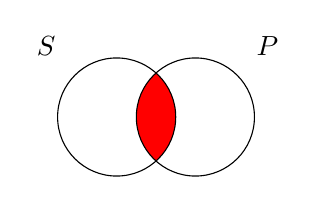
\begin{tikzpicture}
\def\firstcircle{(0,0) circle (.75cm)}
\def\secondcircle{(0:1cm) circle (.75cm)}
%       \begin{scope}[even odd rule]% first circle without the second
%            \clip \secondcircle (-1,-1) rectangle (1,1);
%        \fill[red] \firstcircle;
%        \end{scope}
    \begin{scope}
      \clip \firstcircle;
      \fill[red] \secondcircle;
    \end{scope}
\draw \firstcircle node[outer sep=.66cm, above left] (s) {$S$};
%\node[outer sep=.3cm] (x) {\Large{x}};
%\node[outer sep=.3cm, xshift=.5cm] (x) {\Large{x}};
\draw \secondcircle node[outer sep=.66cm, above right] (p) {$P$};
\end{tikzpicture}\\
$S$: Customers\\
$P$: Things that are mistaken}


\item All cats love catnip.

\answer{
Form: A\\
Quantity: Universal \\
Quality: Affirmative\\

\vspace{.25em}

\noindent 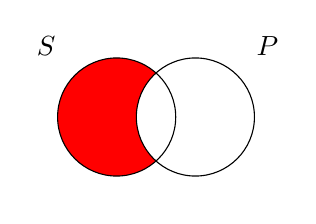
\begin{tikzpicture}
\def\firstcircle{(0,0) circle (.75cm)}
\def\secondcircle{(0:1cm) circle (.75cm)}
       \begin{scope}[even odd rule]% first circle without the second
            \clip \secondcircle (-1,-1) rectangle (1,1);
        \fill[red] \firstcircle;
        \end{scope}
%    \begin{scope}
%      \clip \firstcircle;
%      \fill[red] \secondcircle;
%    \end{scope}
\draw \firstcircle node[outer sep=.66cm, above left] (s) {$S$};
%\node[outer sep=.3cm] (x) {\Large{x}};
%\node[outer sep=.3cm, xshift=.5cm] (x) {\Large{x}};
\draw \secondcircle node[outer sep=.66cm, above right] (p) {$P$};
\end{tikzpicture}\\
$S$: Cats\\
$P$: Things that love catnip
}

\end{exercises}

\noindent \problempart Identify each of the following sentences as A, E, I, or O; state its quantity and quality; and state which terms are distributed. Then draw the Venn Diagram for each.

\begin{exercises}


\item No appeals are rejected.

\item All bagels are boiled.

\item Some employees are late.

\item All forgeries are discovered eventually.

\item Some shirts are purple.

\item Some societies are matriarchal.

\item No sunflowers are blue.

\item Some appetizers are filling. 

\item Some jokes are funny.

\item Some arguments are invalid. 

\end{exercises}

\noindent\problempart Transform the following sentences by switching their quantity, but not their quality.

\textbf{Example}: Some dogs have fleas. \\
\textbf{Answer}: All dogs have fleas.

\begin{exercises}
\item Some trees are not evergreen. \answer{ No trees are evergreen}
\item All smurfs are blue. \answer{ Some smurfs are blue}
\item Some swords are sharp. \answer{ All swords are sharp}
\item Some sweaters are not soft. \answer{ No sweaters are soft}
\item All snails are invertebrates. \answer{Some snails are invertebrates}
\end{exercises}

\noindent\problempart Transform the following sentences by switching their quantity, but not their quality.

\begin{exercises}
\item Some puffins are not large. 
\item Some Smurfs are female.
\item All guitars are stringed instruments. 
\item No lobsters are extraterrestrial.
\item Some metals are alloys 
\end{exercises}

\noindent\problempart Transform the following sentences by switching their quality, but not their quantity.

\textbf{Example}: Some elephants are in zoos. \\
\textbf{Answer}: Some elephants are not in zoos. 

\begin{exercises}
\item Some lobsters are white. \answer{Some lobsters are not white.}

\item Some responsibilities are onerous. \answer{ Some responsibilities are not onerous}

\item No walls are bridges. \answer{All walls are bridges}

\item Some riddles are not clever.\answer{ Some riddles are clever}
 
\item All red things are colored. \answer{No red things are colored}
\end{exercises}

\noindent\problempart Transform the following sentences by switching their quality, but not their quantity.

\begin{exercises}
\item All drums are musical instruments. 
\item No grandsons are female. 
\item Some crimes are felonies.
\item Some airplanes are not commercial. 
\item All scorpions are arachnids. 
\end{exercises}

\noindent\problempart Transform the following sentences by switching both their quality and quantity.

\textbf{Example}: No sharks are virtuous. \\
\textbf{Answer}: Some sharks are virtuous. 

\begin{exercises}
\item No lobsters are vertebrates. \answer{Some lobsters are vertebrates}

\item Some colors are not pastel. \answer{All colors are pastel}

\item All tents are temporary structures.\answer{Some tents are not temporary structures}

\item No goats are bipeds. \answer{Some goats are bipeds}
 
\item Some shirts are plaid.\answer{ No shirts are plaid}
\end{exercises}

\noindent\problempart Transform the following sentences by switching both their quality and quantity.

\begin{exercises}
\item No shirts are pants. 
\item All ducks are birds.  
\item Some possibilities are not likely events.
\item Some raincoats are blue. 
\item Some days are holidays. 
\end{exercises}

% *****************************************************
% * Transforming English into logically structured English.        *
% *****************************************************

\section{Transforming English into Logically Structured English} \label{sec:transformation} 

\newglossaryentry{logically structured English}
{
name=logically structured English,
description={English that has been regimented into a standard form to make its logical structure clear and to remove ambiguity. A stepping stone to full-fledged formal languages.}
}

Because the four basic forms are stated using variables, they have a great deal of generality. We can expand on that generality by showing how many different kinds of English sentences can be transformed into sentences in our four basic forms. We already touched on this a little in section \ref{sec:qcatstatements}, when we look at sentences like ``Thirty percent of Canadians speak French.'' There we saw that the predicate was not explicitly a class. We needed to change ``speak French'' to ``people who speak French.'' In this section, we are going to expand on that to show how ordinary English sentences can be transformed into something we will call ``logically structured English.'' \textsc{\gls{logically structured English}} \label{def:LSE} is English that has been put into a standardized form that allows us to see its logical structure more clearly and removes ambiguity.  Doing this is a step towards the creation of formal languages, which we will start doing in Chapter \ref{chap:SL}. 

Transforming English sentences into logically structured English is fundamentally a matter of understanding the meaning of the English sentence and then finding the logically structured English statements with the same or similar meaning. Sometimes this will require judgment calls. English, like any natural  language, is fraught with ambiguity. One of our goals with logically structured English is to reduce the amount of ambiguity. Clarifying ambiguous sentences will always require making judgments that can be questioned. Things will only get harder when we start using full blown formal languages in Chapter \ref{chap:SL}, which are supposed to be completely free of ambiguity.

\newglossaryentry{standard form for a categorical statement}
{
name=standard form for a categorical statement,
description={A categorical statement that has been put into logically structured English, with the following elements in the following order: (1) The quantifiers ``all,'' ``some,'' or ``no''; (2) the subject term; (3) the copula ``are'' or ``are not''; and (4) the predicate term.}
}


To transform a quantified categorical statement into logically structured English, we have to put all of its elements in a fixed order and be sure they are all of the right type. All statements must begin with the quantifies ``All'' or ``Some'' or the negated quantifier ``No.'' Next comes the subject term, which must be a plural noun, a noun phrase, or a variable that stands for any plural noun or noun phrase. Then comes the copula ``are'' or the negated copula ``are not.'' Last is the predicate term, which must also be a plural noun or noun phrase. We also specify that you can only say ``are not'' with the quantifier ``some,'' that way the universal negative statement is always phrased ``No $S$ are $P$,'' not ``All S are not $P$.'' Taken together, these criteria define the \textsc{\gls{standard form for a categorical statement}} in logically structured English. \label{def:standard_form_cat_statement}

The subsections below identify different kinds of changes you might need to make to put a statement into logically structured English. Sometimes translating a sentence will require using multiple changes.

\subsection{Nonstandard Verbs}
\label{subsec:nonstandard_verbs}
In section \ref{sec:qcatstatements} we saw that ``Some Canadians speak French'' has a verb phrase ``speaks French'' instead of a copula and a plural noun phrase. To transform these sentences into logically structured English, you need to add the copula and turn all the terms into plural nouns or plural noun phrases. 

Below are some examples


\begin{longtabu}{p{.5\linewidth}p{.5\linewidth}}
\underline{English} &
\underline{Logically Structured English} \\
\endhead 
No cats bark. &
No cats are animals that bark.  \\ 

All birds can fly. &
All birds are animals that can fly.  \\

Some thoughts should be left unsaid. &
Some thoughts are things that should be left unsaid. 
\end{longtabu}



Adding a plural noun phrase means you have to come up with some category, like ``people'' or ``animals.'' When in doubt, you can always use the most general category, ``things.'' 

\subsection{Implicit Noun Phrases}

Sometimes you just have an adjective for the predicate, and you need to turn it into a noun, as in the examples below. 


\begin{longtabu}{p{.5\linewidth}p{.5\linewidth}}
\underline{English} &
\underline{Logically Structured English}  \\
\endhead 
Some roses are red. &
Some roses are red flowers. \\

Football players are strong. &
All football players are strong persons. \\

Some names are hurtful. &
Some names are hurtful things.
\end{longtabu}

Again, you will have to come up with a category for the predicate, and when it doubt, you can just use ``things.''



\subsection{Unexpressed Quantifiers}

Sometimes categorical generalizations come without an explicit quantifier, which you need to add. 


\begin{longtabu}{p{.5\linewidth}p{.5\linewidth}}
\underline{English} &
\underline{Logically Structured English} \\
\endhead 
Boots are footwear. &
All boots are footwear.\\

Giraffes are tall. &
All giraffes are tall things.\\

A dog is not a cat. & 
No dogs are cats.\\

A lion is a fierce creature. &
All lions are fierce creatures.\\

\end{longtabu}

Notice that in the second sentence we had to make two changes, adding both the words ``All'' and ``things.''

In the last two sentences, the indefinite article ``a'' is being used to create a kind of generic sentence. Not all sentences using the indefinite article work this way. If a story begins ``A man is walking down the street,'' it is not talking about all men generically. It is introducing some specific man. For this kind of  statement, see the subsection on singular propositions. You will have to use your good judgment and understanding of context to know how the indefinite article is being used.

\subsection{Nonstandard Quantifiers}
\label{subsec:nonstandard_quantifiers}
English has many alternate ways of saying ``all'' and ``some.'' You need to change these when translating to logically structured English. 

\begin{longtabu}{p{.5\linewidth}p{.5\linewidth}}
\underline{English} &
\underline{Logically Structured English} \\
\endhead 
Every day is a blessing. &
All days are blessings. \\

Whatever is a dog is not a cat. &
No dogs are cats. \\

Not a single dog is a cat. &
No dogs are cats. \\

There are Americans that are doctors. &
Some Americans are doctors. \\

Someone in America is a doctor. &
Some Americans are doctors. \\

At least a few Americans are doctors.&
Some Americans are doctors. \\

Not everyone who is an adult is a logician. &
Some adults are not logicians. \\

Most people with a PhD in psychology are female. &
Some people with a PhD in psychology are female. \\

Among the things that Sylvia inherited was a large mirror &
Some things that Sylvia inherited were large mirrors
\end{longtabu}

Notice in the last case we are losing quite a bit of information when we transform the sentence into logically structured English. ``Most'' means more that fifty percent, while ``some'' could be any percentage less than a hundred. This is simply a price we have to pay in creating a standard logical form. As we will see when we move to constructing artificial languages in Chapter \ref{chap:SL}, no logical language has the expressive richness of a natural language. 

\subsection{Singular Propositions}
\label{subsec:singular_propositions}
Aristotle treated sentences about individual things, like specific people, differently than either general or particular categorical statements. A statement like ``Socrates is mortal,'' for Aristotle, was neither A, E, I, nor O. We can expand the power of logically structured English by bringing these kind of singular propositions into our system of categorical propositions. Using phrases like ``All things identical to\ldots'' we can turn singular terms into general ones. 

\begin{longtabu}{p{.5\linewidth}p{.5\linewidth}}
\underline{English} &
\underline{Logically Structured English} \\
\endhead 
Socrates is mortal.&
All persons identical with Socrates are mortal. \\

The Empire State Building is tall. &
All things identical to The Empire State Building are tall things. \\

Ludwig was not happy. &
No persons identical with Ludwig are happy. \\

A man is walking down the street. &
Some men are things that are walking down the street.
\end{longtabu}

\subsection{Adverbs and Pronouns}

In English we use specific adverbs like ``everywhere'' and ``always'' to create quantified statements about place and time. We can transform these into logically structured English by talking about ``all places'' or ``all times''  and things like that. English also has specific pronouns for quantified statements about people or things, such as ``everyone'' or ``nothing.'' 


\tabulinesep=1.25ex
\begin{longtabu}{p{.5\linewidth}p{.5\linewidth}}
\underline{English} &
\underline{Logically Structured English} \\
\endhead 
``Whenever you need me, I'll be there.'' -- Michael Jackson &
All times that you need me are times that I will be there. \\

``We are never, ever, ever getting back together.'' -- Taylor Swift &
No times are times when we will get back together.\\

``Whoever fights with monsters should be careful lest he thereby become a monster.'' --Friedrich Nietzsche & 
All persons who fight with monsters are persons who should be careful lest they become a monster.\\

``What does not destroy me, makes me stronger.'' --Friedrich Nietzsche & 
All things that do not destroy me are things that make me stronger. 
 

\end{longtabu}
\tabulinesep=.75ex

%
%\subsection{``It Is False That''}
%
%In English, we can say ``It is false that \ldots'' or ``It is not the case that \ldots'' to indicate that a statement is false. A lawyer, for instance, might say ``It is not the case that you signed the consent form before the doctor did the procedure.'' In logically structured English, we can make these simpler by converting the negated proposition to its contradictory. A negated A statement will become an O statement, and vice versa. Likewise a negating E statement will become and I statement, and vice versa. See the examples below. This time we have marked their form A, E, I or O, with a ``not-'' for the cases where they are negated. 
%
%\begin{tabu}{p{.5\linewidth}p{.5\linewidth}}
%\underline{English} &
%\underline{Logically Structured English} \\
%
%\textbf{not-A}: It is not the case that all dogs are pets &
%\textbf{O}: Some dogs are not pets.\\
%
%\textbf{not-I}: It is not the case that some dogs are reptiles &
%\textbf{E}: No dogs are reptiles\\
%
%\textbf{not-E}: It is not the case that no dogs are pets &
%\textbf{I}: Some dogs are pets \\
%
%\textbf{not-O}: It is not the case that some dogs are not mammals &
%\textbf{A}: All dogs are mammals. 
%\end{tabu}


\subsection{Conditional Statements}

A conditional is a statement of the form ``If \ldots then \ldots.'' They will become a big focus of our attention starting in Chapter \ref{chap:SL} when we begin introducing modern formal languages. They are not given special treatment in the Aristotelian tradition, however. Instead, where we can, we just treat them as categorical generalizations:

\begin{longtabu}{p{.5\linewidth}p{.5\linewidth}}
\underline{English} &
\underline{Logically Structured English} \\
\endhead 
If something is a cat, then it is a feline. &
All cats are feline.\\

If something is a dog, then it's not a cat. &
No dogs are cats. \\
\end{longtabu}


\subsection{Exclusive Propositions}

Phrases like ``only,'' ``none but,'' or ``none except'' are used in English to create exclusive propositions. They are applied to the predicate term and exclude everything but the predicate term from the subject term. 

\begin{longtabu}{p{.5\linewidth}p{.5\linewidth}}
\underline{English} &
\underline{Logically Structured English} \\
\endhead 
Only people over 21 may drink. &
All people who drink are over 21.\\

No one, except those with a ticket, may enter the theater. &
All people who enter the theater have a ticket. \\

None but the strong survive. &
All people who survive are strong people. \\
\end{longtabu}

The important thing to see here is that words like ``only'' are actually modifying the predicate, and not the subject. So when you translate them into logically structured English, the order of the words often gets turned around. In ``only people over 21 may drink'' the predicate is actually ``people over 21.''


\subsection{``The Only''}

Sentences with ``The only'' are a little different than sentences that just have ``only'' in them. The sentence ``Humans are the only animals that talk on cell phones'' should be translated as ``All animals who talk on cell phones are humans.'' In this sentence, ``the only'' introduces the subject, rather than the predicate. 

\begin{longtabu}{p{.5\linewidth}p{.5\linewidth}}
\underline{English} &
\underline{Logically Structured English} \\
\endhead 
Humans are the only animals who talk on cell phones. &
All animals who talk on cell phones are human.\\

Shrews are the only venomous mammal in North America. &
All venomous mammals in North America are shrews.\\

\end{longtabu}

%%%%%%%%%% practice problems %%%%%%%%%%%%

\practiceproblems
\noindent\problempart Transform the following into logically structured English; identify it as A, E, I, or O; and provide the appropriate Venn diagram.


\begin{longtabu}{p{.1\linewidth}p{.9\linewidth}}
\textbf{Example}: & If you can't stand the heat, get out of the kitchen \\
\textbf{Answer}:  & All people who cannot stand the heat are people who should get out of the kitchen. \\
& Form: A\\
&
\noindent 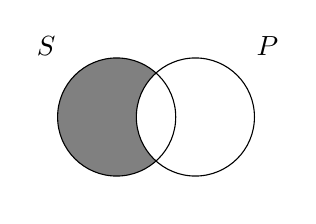
\begin{tikzpicture}
\def\firstcircle{(0,0) circle (.75cm)}
\def\secondcircle{(0:1cm) circle (.75cm)}
     \begin{scope}[shift={(4cm,0cm)}]
        \begin{scope}[even odd rule]% first circle without the second
            \clip \secondcircle (-1,-1) rectangle (1,1);
        \fill[gray] \firstcircle;
        \end{scope}
\draw \firstcircle node[outer sep=.66cm, above left] (s) {$S$};
\draw \secondcircle node[outer sep=.66cm, above right] (p) {$P$};
        \end{scope}

\end{tikzpicture}\\
& $S$: People who can't stand the heat\\
& $P$: People who should get out of the kitchen

\end{longtabu}

\begin{exercises}
\item Cats are predators.\answer{\\
All cats are predators. \\
Form: A \\

\noindent 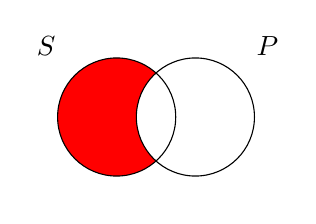
\begin{tikzpicture}
\def\firstcircle{(0,0) circle (.75cm)}
\def\secondcircle{(0:1cm) circle (.75cm)}
     \begin{scope}[shift={(4cm,0cm)}]
        \begin{scope}[even odd rule]% first circle without the second
            \clip \secondcircle (-1,-1) rectangle (1,1);
        \fill[red] \firstcircle;
        \end{scope}
\draw \firstcircle node[outer sep=.66cm, above left] (s) {$S$};
\draw \secondcircle node[outer sep=.66cm, above right] (p) {$P$};
        \end{scope}

\end{tikzpicture}\\
$S$: Cats\\
$P$: Predators
}

\item If something is worth doing, it is worth doing well. \answer{\\
All things that are worth doing are things that are worth doing well. \\
Form: A \\

\noindent 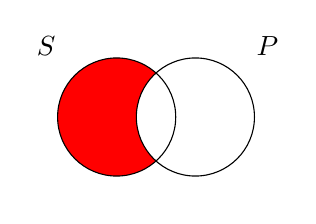
\begin{tikzpicture}
\def\firstcircle{(0,0) circle (.75cm)}
\def\secondcircle{(0:1cm) circle (.75cm)}
     \begin{scope}[shift={(4cm,0cm)}]
        \begin{scope}[even odd rule]% first circle without the second
            \clip \secondcircle (-1,-1) rectangle (1,1);
        \fill[red] \firstcircle;
        \end{scope}
\draw \firstcircle node[outer sep=.66cm, above left] (s) {$S$};
\draw \secondcircle node[outer sep=.66cm, above right] (p) {$P$};
        \end{scope}

\end{tikzpicture}\\
$S$: Things that are worth doing \\
$P$: Things that are worth doing well.
}

\item Some chimpanzees know sign language. \answer{\\
Some chimpanzees are things that know sign language. \\
Form: I \\
\noindent 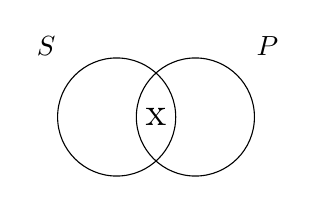
\begin{tikzpicture}
\def\firstcircle{(0,0) circle (.75cm)}
\def\secondcircle{(0:1cm) circle (.75cm)}
%        \begin{scope}[even odd rule]% first circle without the second
%            \clip \secondcircle (-1,-1) rectangle (1,1);
%        \fill[red] \firstcircle;
%        \end{scope}
%    \begin{scope}
%      \clip \firstcircle;
%      \fill[red] \secondcircle;
%    \end{scope}
\draw \firstcircle node[outer sep=.66cm, above left] (s) {$S$};
%\node[outer sep=.3cm] (x) {\Large{x}};
\node[outer sep=.3cm, xshift=.5cm] (x) {\Large{x}};
\draw \secondcircle node[outer sep=.66cm, above right] (p) {$P$};
\end{tikzpicture}\\
$S$: Chimpanzees \\
$P$: Things that know sign language.
}

\item All dogs are loyal. \answer{\\
All dogs are things that are loyal. \\
Form: A \\
\noindent 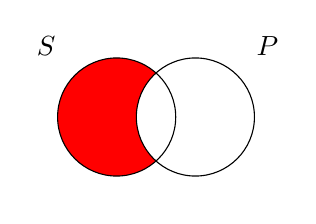
\begin{tikzpicture}
\def\firstcircle{(0,0) circle (.75cm)}
\def\secondcircle{(0:1cm) circle (.75cm)}
        \begin{scope}[even odd rule]% first circle without the second
            \clip \secondcircle (-1,-1) rectangle (1,1);
        \fill[red] \firstcircle;
        \end{scope}
%    \begin{scope}
%      \clip \firstcircle;
%      \fill[red] \secondcircle;
%    \end{scope}
\draw \firstcircle node[outer sep=.66cm, above left] (s) {$S$};
%\node[outer sep=.3cm] (x) {\Large{x}};
%\node[outer sep=.3cm, xshift=.5cm] (x) {\Large{x}};
\draw \secondcircle node[outer sep=.66cm, above right] (p) {$P$};
\end{tikzpicture}\\
$S$: Dogs \\
$P$: Things that are loyal.
}

\item Monotremes are the only egg-laying mammals.\answer{\\
All egg-laying mammals are monotremes. \\
Form: A \\
\noindent 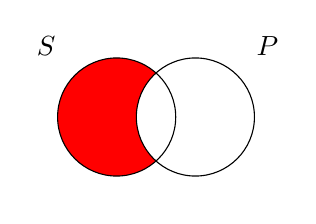
\begin{tikzpicture}
\def\firstcircle{(0,0) circle (.75cm)}
\def\secondcircle{(0:1cm) circle (.75cm)}
        \begin{scope}[even odd rule]% first circle without the second
            \clip \secondcircle (-1,-1) rectangle (1,1);
        \fill[red] \firstcircle;
        \end{scope}
%    \begin{scope}
%      \clip \firstcircle;
%      \fill[red] \secondcircle;
%    \end{scope}
\draw \firstcircle node[outer sep=.66cm, above left] (s) {$S$};
%\node[outer sep=.3cm] (x) {\Large{x}};
%\node[outer sep=.3cm, xshift=.5cm] (x) {\Large{x}};
\draw \secondcircle node[outer sep=.66cm, above right] (p) {$P$};
\end{tikzpicture}\\
$S$: Egg-laying mammals \\
$P$: Monotremes\\
\vspace{11pt}
Remember that ``the only'' introduces the subject, not the predicate. See page 72
}

\item Whenever a bell rings, an angel gets its wings. \answer{\\
All times that a bell rings are times that an angel gets its wings. \\
Form: A \\
\noindent 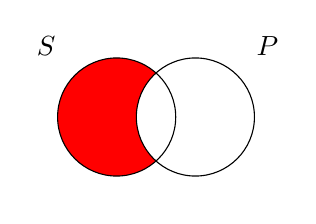
\begin{tikzpicture}
\def\firstcircle{(0,0) circle (.75cm)}
\def\secondcircle{(0:1cm) circle (.75cm)}
        \begin{scope}[even odd rule]% first circle without the second
            \clip \secondcircle (-1,-1) rectangle (1,1);
        \fill[red] \firstcircle;
        \end{scope}
%    \begin{scope}
%      \clip \firstcircle;
%      \fill[red] \secondcircle;
%    \end{scope}
\draw \firstcircle node[outer sep=.66cm, above left] (s) {$S$};
%\node[outer sep=.3cm] (x) {\Large{x}};
%\node[outer sep=.3cm, xshift=.5cm] (x) {\Large{x}};
\draw \secondcircle node[outer sep=.66cm, above right] (p) {$P$};
\end{tikzpicture}\\
$S$: Times that a bell rings \\
$P$: Times that an angel gets its wings\\
\vspace{11pt}
Remember that words like ``whenever'' and ``where ever'' are really specialized quantifiers for places and times, and need to be replaced by ``all places'' and ``all times.'' See page 71.
}


\item At least one person in this room is a liar. \answer{\\
Some people in this room are liars. \\
Form: I \\
\noindent 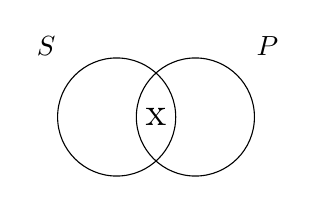
\begin{tikzpicture}
\def\firstcircle{(0,0) circle (.75cm)}
\def\secondcircle{(0:1cm) circle (.75cm)}
%        \begin{scope}[even odd rule]% first circle without the second
%            \clip \secondcircle (-1,-1) rectangle (1,1);
%        \fill[red] \firstcircle;
%        \end{scope}
%    \begin{scope}
%      \clip \firstcircle;
%      \fill[red] \secondcircle;
%    \end{scope}
\draw \firstcircle node[outer sep=.66cm, above left] (s) {$S$};
%\node[outer sep=.3cm] (x) {\Large{x}};
\node[outer sep=.3cm, xshift=.5cm] (x) {\Large{x}};
\draw \secondcircle node[outer sep=.66cm, above right] (p) {$P$};
\end{tikzpicture}\\
$S$: People in this room \\
$P$: Liars\\
\vspace{11pt}
}


\item Only natural born citizens can be president of the United States.\answer{\\
All presidents of the United States are natural born citizens. \\
Form: A \\
\noindent 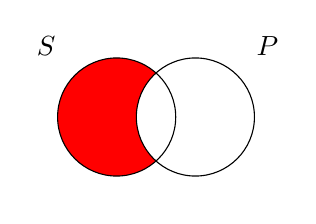
\begin{tikzpicture}
\def\firstcircle{(0,0) circle (.75cm)}
\def\secondcircle{(0:1cm) circle (.75cm)}
        \begin{scope}[even odd rule]% first circle without the second
            \clip \secondcircle (-1,-1) rectangle (1,1);
        \fill[red] \firstcircle;
        \end{scope}
%    \begin{scope}
%      \clip \firstcircle;
%      \fill[red] \secondcircle;
%    \end{scope}
\draw \firstcircle node[outer sep=.66cm, above left] (s) {$S$};
%\node[outer sep=.3cm] (x) {\Large{x}};
%\node[outer sep=.3cm, xshift=.5cm] (x) {\Large{x}};
\draw \secondcircle node[outer sep=.66cm, above right] (p) {$P$};
\end{tikzpicture}\\
$S$: Presidents of the United States\\
$P$: Natural born citizens\\
\vspace{11pt}
}

\item Gottlob Frege suffered from severe depression. \answer{\\
All people identical with Gottlob Frege are people who suffer from severe depression. \\
Form: A \\
\noindent 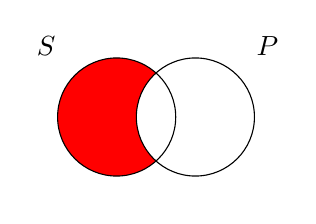
\begin{tikzpicture}
\def\firstcircle{(0,0) circle (.75cm)}
\def\secondcircle{(0:1cm) circle (.75cm)}
        \begin{scope}[even odd rule]% first circle without the second
            \clip \secondcircle (-1,-1) rectangle (1,1);
        \fill[red] \firstcircle;
        \end{scope}
%    \begin{scope}
%      \clip \firstcircle;
%      \fill[red] \secondcircle;
%    \end{scope}
\draw \firstcircle node[outer sep=.66cm, above left] (s) {$S$};
%\node[outer sep=.3cm] (x) {\Large{x}};
%\node[outer sep=.3cm, xshift=.5cm] (x) {\Large{x}};
\draw \secondcircle node[outer sep=.66cm, above right] (p) {$P$};
\end{tikzpicture}\\
$S$: People identical with Gottlob Frege\\
$P$: People who suffer from severe depression\\
}

\item ``Anyone who ever had a heart, wouldn't turn around and break it.'' --Lou Reed. \answer{\\
No things who ever had a heart are things that would turn around and break it. \\
Form: E \\
\noindent 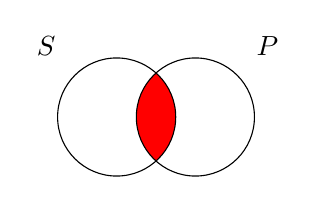
\begin{tikzpicture}
\def\firstcircle{(0,0) circle (.75cm)}
\def\secondcircle{(0:1cm) circle (.75cm)}
%        \begin{scope}[even odd rule]% first circle without the second
%            \clip \secondcircle (-1,-1) rectangle (1,1);
%        \fill[red] \firstcircle;
%        \end{scope}
    \begin{scope}
      \clip \firstcircle;
      \fill[red] \secondcircle;
    \end{scope}
\draw \firstcircle node[outer sep=.66cm, above left] (s) {$S$};
%\node[outer sep=.3cm] (x) {\Large{x}};
%\node[outer sep=.3cm, xshift=.5cm] (x) {\Large{x}};
\draw \secondcircle node[outer sep=.66cm, above right] (p) {$P$};
\end{tikzpicture}\\
$S$: Things who ever had a heart\\
$P$: Things that would turn around a break it\\
}

\end{exercises}


\noindent\problempart Transform the following into logically structured English, and identify it as A, E, I, or O.

\begin{exercises}
\item If a muffin has frosting, then it is a cupcake.
\item ``Anyone who ever played a part, wouldn't turn around and hate it.'' --Lou Reed.
\item Seahorses are the only fish species in which the male carries the eggs. 
\item Seahorses are animals that mate for life.
\item Few dogs are fans of classical music.
\item Ruth Barcan Marcus was a member of the Yale faculty.
\item Only zombies are brain eaters.
\item Some logicians are not mentally ill
\item Some birds eat fish.
\end{exercises}

\noindent\problempart Transform the following into logically structured English and identify it as A, E, I, or O. Some problems will require multiple transformations.

\begin{longtabu}{p{.1\linewidth}p{.9\linewidth}}
\textbf{Example}: & Bertrand Russell was married four times. \\
\textbf{Answer}:  & All people who are identical to Bertrand Russell are people who were married four times. \\
& Form: A\\
&
\noindent 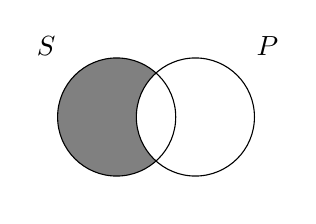
\begin{tikzpicture}
\def\firstcircle{(0,0) circle (.75cm)}
\def\secondcircle{(0:1cm) circle (.75cm)}
     \begin{scope}[shift={(4cm,0cm)}]
        \begin{scope}[even odd rule]% first circle without the second
            \clip \secondcircle (-1,-1) rectangle (1,1);
        \fill[gray] \firstcircle;
        \end{scope}
\draw \firstcircle node[outer sep=.66cm, above left] (s) {$S$};
\draw \secondcircle node[outer sep=.66cm, above right] (p) {$P$};
        \end{scope}
\end{tikzpicture}\\
& $S$: People who are identical to Bertrand Russell\\
& $P$: People who were married four times
\end{longtabu}

\begin{exercises}

\item Many logicians work in computer science. \answer{\\
Some logicians are people who work in computer science. \\
Form: E \\
\noindent 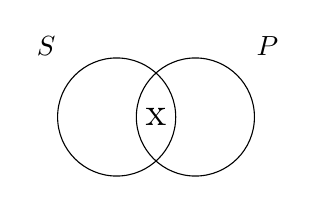
\begin{tikzpicture}
\def\firstcircle{(0,0) circle (.75cm)}
\def\secondcircle{(0:1cm) circle (.75cm)}
%        \begin{scope}[even odd rule]% first circle without the second
%            \clip \secondcircle (-1,-1) rectangle (1,1);
%        \fill[red] \firstcircle;
%        \end{scope}
%    \begin{scope}
%      \clip \firstcircle;
%      \fill[red] \secondcircle;
%    \end{scope}
\draw \firstcircle node[outer sep=.66cm, above left] (s) {$S$};
%\node[outer sep=.3cm] (x) {\Large{x}};
\node[outer sep=.3cm, xshift=.5cm] (x) {\Large{x}};
\draw \secondcircle node[outer sep=.66cm, above right] (p) {$P$};
\end{tikzpicture}\\
$S$: Logicians\\
$P$: Things that work in computer science\\
}


\item Ludwig Wittgenstein severed in the Austro-Hungarian Army in World War I.\answer{\\
All things identical to Ludwig Wittgenstein are things that served in the Austro-Hungarian Army in World War I \\
Form: A \\
\noindent 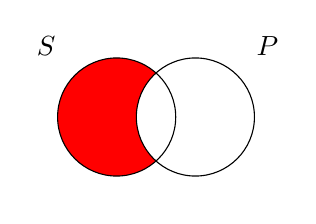
\begin{tikzpicture}
\def\firstcircle{(0,0) circle (.75cm)}
\def\secondcircle{(0:1cm) circle (.75cm)}
        \begin{scope}[even odd rule]% first circle without the second
            \clip \secondcircle (-1,-1) rectangle (1,1);
        \fill[red] \firstcircle;
        \end{scope}
%    \begin{scope}
%      \clip \firstcircle;
%      \fill[red] \secondcircle;
%    \end{scope}
\draw \firstcircle node[outer sep=.66cm, above left] (s) {$S$};
%\node[outer sep=.3cm] (x) {\Large{x}};
%\node[outer sep=.3cm, xshift=.5cm] (x) {\Large{x}};
\draw \secondcircle node[outer sep=.66cm, above right] (p) {$P$};
\end{tikzpicture}\\
$S$: Things identical to Ludwig Wittgenstein\\
$P$: Things that served int he Austro-Hungarian Army in WWI\\
}

\item Humans can be found everywhere on Earth.\answer{\\
All humans are things that can be found everywhere on Earth. \\
Form: A \\
\noindent 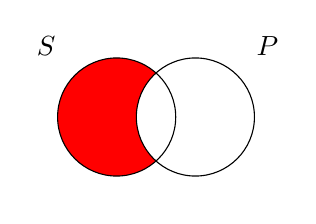
\begin{tikzpicture}
\def\firstcircle{(0,0) circle (.75cm)}
\def\secondcircle{(0:1cm) circle (.75cm)}
        \begin{scope}[even odd rule]% first circle without the second
            \clip \secondcircle (-1,-1) rectangle (1,1);
        \fill[red] \firstcircle;
        \end{scope}
%    \begin{scope}
%      \clip \firstcircle;
%      \fill[red] \secondcircle;
%    \end{scope}
\draw \firstcircle node[outer sep=.66cm, above left] (s) {$S$};
%\node[outer sep=.3cm] (x) {\Large{x}};
%\node[outer sep=.3cm, xshift=.5cm] (x) {\Large{x}};
\draw \secondcircle node[outer sep=.66cm, above right] (p) {$P$};
\end{tikzpicture}\\
$S$: Humans\\
$P$: Things that can be found everywhere on Earth\\
}

\item Cats are crepuscular. \answer{\\
All cats are crepuscular. \\
Form: A \\
\noindent 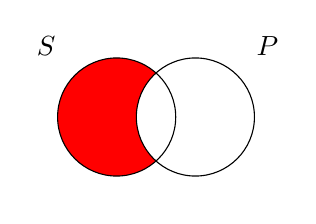
\begin{tikzpicture}
\def\firstcircle{(0,0) circle (.75cm)}
\def\secondcircle{(0:1cm) circle (.75cm)}
        \begin{scope}[even odd rule]% first circle without the second
            \clip \secondcircle (-1,-1) rectangle (1,1);
        \fill[red] \firstcircle;
        \end{scope}
%    \begin{scope}
%      \clip \firstcircle;
%      \fill[red] \secondcircle;
%    \end{scope}
\draw \firstcircle node[outer sep=.66cm, above left] (s) {$S$};
%\node[outer sep=.3cm] (x) {\Large{x}};
%\node[outer sep=.3cm, xshift=.5cm] (x) {\Large{x}};
\draw \secondcircle node[outer sep=.66cm, above right] (p) {$P$};
\end{tikzpicture}\\
$S$: Cats\\
$P$: Things that are crepuscular\\
}

\item Grover Cleveland was the only president to serve two nonconsecutive terms. \answer{\\
All presidents who served two nonconsecutive terms are things identical to Grover Cleveland. \\
Form: A \\
\noindent 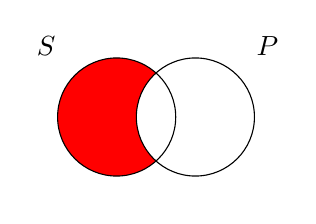
\begin{tikzpicture}
\def\firstcircle{(0,0) circle (.75cm)}
\def\secondcircle{(0:1cm) circle (.75cm)}
        \begin{scope}[even odd rule]% first circle without the second
            \clip \secondcircle (-1,-1) rectangle (1,1);
        \fill[red] \firstcircle;
        \end{scope}
%    \begin{scope}
%      \clip \firstcircle;
%      \fill[red] \secondcircle;
%    \end{scope}
\draw \firstcircle node[outer sep=.66cm, above left] (s) {$S$};
%\node[outer sep=.3cm] (x) {\Large{x}};
%\node[outer sep=.3cm, xshift=.5cm] (x) {\Large{x}};
\draw \secondcircle node[outer sep=.66cm, above right] (p) {$P$};
\end{tikzpicture}\\
$S$: Presidents who served two nonconsecutive terms \\
$P$: Things identical to Grover Cleveland\\
}

\item Grover Cleveland was the only president named ``Grover.'' \answer{\\
All presidents named Grover are things identical to Grover Cleveland. \\
Form: A \\
\noindent 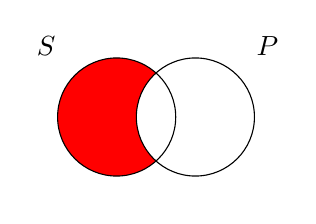
\begin{tikzpicture}
\def\firstcircle{(0,0) circle (.75cm)}
\def\secondcircle{(0:1cm) circle (.75cm)}
        \begin{scope}[even odd rule]% first circle without the second
            \clip \secondcircle (-1,-1) rectangle (1,1);
        \fill[red] \firstcircle;
        \end{scope}
%    \begin{scope}
%      \clip \firstcircle;
%      \fill[red] \secondcircle;
%    \end{scope}
\draw \firstcircle node[outer sep=.66cm, above left] (s) {$S$};
%\node[outer sep=.3cm] (x) {\Large{x}};
%\node[outer sep=.3cm, xshift=.5cm] (x) {\Large{x}};
\draw \secondcircle node[outer sep=.66cm, above right] (p) {$P$};
\end{tikzpicture}\\
$S$: Presidents named ``Grover''\\
$P$: Things identical to Grover Cleveland\\
}



\item The band's only singer also plays guitar. \answer{\\
All things identical to the singer of the band are things that play guitar. \\
Form: A \\
\noindent 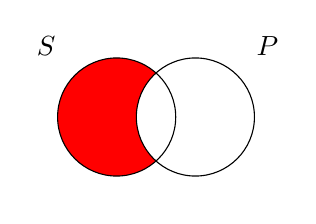
\begin{tikzpicture}
\def\firstcircle{(0,0) circle (.75cm)}
\def\secondcircle{(0:1cm) circle (.75cm)}
        \begin{scope}[even odd rule]% first circle without the second
            \clip \secondcircle (-1,-1) rectangle (1,1);
        \fill[red] \firstcircle;
        \end{scope}
%    \begin{scope}
%      \clip \firstcircle;
%      \fill[red] \secondcircle;
%    \end{scope}
\draw \firstcircle node[outer sep=.66cm, above left] (s) {$S$};
%\node[outer sep=.3cm] (x) {\Large{x}};
%\node[outer sep=.3cm, xshift=.5cm] (x) {\Large{x}};
\draw \secondcircle node[outer sep=.66cm, above right] (p) {$P$};
\end{tikzpicture}\\
$S$: Things identical to the singer of the band\\
$P$: Things that play guitar\\
}

\item If a dog has a collar, it is someone's pet.\answer{\\
All dogs that have a collar are things that are someone's pet.\\
Form: A \\
\noindent 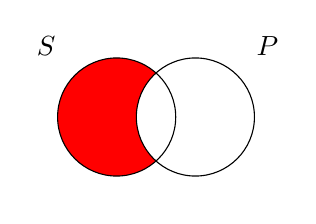
\begin{tikzpicture}
\def\firstcircle{(0,0) circle (.75cm)}
\def\secondcircle{(0:1cm) circle (.75cm)}
        \begin{scope}[even odd rule]% first circle without the second
            \clip \secondcircle (-1,-1) rectangle (1,1);
        \fill[red] \firstcircle;
        \end{scope}
%    \begin{scope}
%      \clip \firstcircle;
%      \fill[red] \secondcircle;
%    \end{scope}
\draw \firstcircle node[outer sep=.66cm, above left] (s) {$S$};
%\node[outer sep=.3cm] (x) {\Large{x}};
%\node[outer sep=.3cm, xshift=.5cm] (x) {\Large{x}};
\draw \secondcircle node[outer sep=.66cm, above right] (p) {$P$};
\end{tikzpicture}\\
$S$: Dogs that have a collar\\
$P$: Things that are someone's pet. \\
}

\item Only the basketball players in the class were tall. \answer{\\
All tall people in the class were basketball players\\
Form: A \\
\noindent 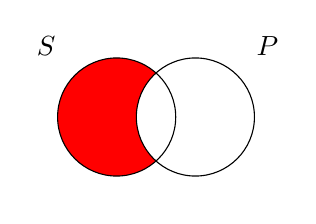
\begin{tikzpicture}
\def\firstcircle{(0,0) circle (.75cm)}
\def\secondcircle{(0:1cm) circle (.75cm)}
        \begin{scope}[even odd rule]% first circle without the second
            \clip \secondcircle (-1,-1) rectangle (1,1);
        \fill[red] \firstcircle;
        \end{scope}
%    \begin{scope}
%      \clip \firstcircle;
%      \fill[red] \secondcircle;
%    \end{scope}
\draw \firstcircle node[outer sep=.66cm, above left] (s) {$S$};
%\node[outer sep=.3cm] (x) {\Large{x}};
%\node[outer sep=.3cm, xshift=.5cm] (x) {\Large{x}};
\draw \secondcircle node[outer sep=.66cm, above right] (p) {$P$};
\end{tikzpicture}\\
$S$: All tall people in the class\\
$P$: Basketball players\\
}

\item If you study, then you will pass the test.\answer{\\
All things that study are things that will pass the test. \\
Form: A \\
\noindent 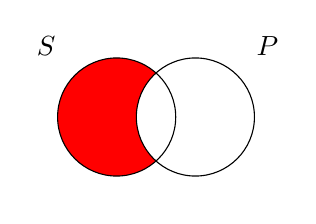
\begin{tikzpicture}
\def\firstcircle{(0,0) circle (.75cm)}
\def\secondcircle{(0:1cm) circle (.75cm)}
        \begin{scope}[even odd rule]% first circle without the second
            \clip \secondcircle (-1,-1) rectangle (1,1);
        \fill[red] \firstcircle;
        \end{scope}
%    \begin{scope}
%      \clip \firstcircle;
%      \fill[red] \secondcircle;
%    \end{scope}
\draw \firstcircle node[outer sep=.66cm, above left] (s) {$S$};
%\node[outer sep=.3cm] (x) {\Large{x}};
%\node[outer sep=.3cm, xshift=.5cm] (x) {\Large{x}};
\draw \secondcircle node[outer sep=.66cm, above right] (p) {$P$};
\end{tikzpicture}\\
$S$: All things who study \\
$P$: All things who pass the test\\
}

\end{exercises}


\noindent\problempart Transform the following into logically structured English, and identify it as A, E, I, or O. Some problems will require multiple transformations.

\begin{exercises}
\item People have walked on the moon at least once. 
\item Basketball players are tall.
\item Most senior citizens vote.
\item If a bird is a crow, then it is very intelligent. 
\item Whoever ate the last cookie is in trouble.
\item ``Euclid alone has looked on Beauty bare.'' --Edna St. Vincent Millay.
\item If something is a dog, then it is man's best friend.
\item More than a few students will fail the test.
\item Mercury is the only metal that is liquid at room temperature. 
\item Bertrand Russell was married four times.
\end{exercises}

%Something is a dog only if it's not a cat.
%Dogs are not cats. &
%No dogs are cats.\\

% *****************************************
% * Conversion, Obversion, and Contraposition   *
% *****************************************

\section{Conversion, Obversion, and Contraposition}
\label{sec:conv_obv_cont}
Now that we have shown the wide range of statements that can be represented in our four standard logical forms A, E, I, and O, it is time to begin constructing arguments with them. The arguments we are going to look at are sometimes called ``immediate inferences'' because they only have one premise. We are going to learn to identify some valid forms of these one-premise arguments by looking at ways you can transform a true sentence that maintain its truth value. For instance, ``No dogs are reptiles'' and ``No reptiles are dogs'' have the same truth value and basically mean the same thing. On the other hand if you change ``All dogs are mammals'' into ``All mammals are dogs'' you turn a true sentence into a false one. In this section we are going to look at three ways of transforming categorical statements---conversion, obversion, and contraposition---and use Venn diagrams to determine whether these transformations also lead to a change in truth value. From there we can identify valid argument forms. 

\subsection{Conversion}

\newglossaryentry{conversion}
{
name=conversion,
description={The process of changing a sentence by reversing the subject and predicate.}
}


The two examples in the last paragraph are examples of conversion. \textsc{\gls{conversion}} \label{defConversion} is the process of transforming a categorical statement by switching the subject and the predicate. When you convert a statement, it keeps its form---an A statement remains an A statement, an E statement remains an E statement---however it might change its truth value.  The Venn diagrams in Figure \ref{fig:conversion} illustrate this.

\begin{figure}
\begin{mdframed}[style=mytablebox]
\begin{tabu}{p{.5\linewidth}p{.5\linewidth}}

\underline{Original Statement}

&

\underline{Converse} \\

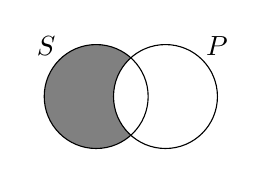
\begin{tikzpicture}
\def\firstcircle{(0,0) circle (.66cm)}
\def\secondcircle{(0:.88cm) circle (.66cm)}
     \begin{scope}[shift={(4cm,0cm)}]
        \begin{scope}[even odd rule]% first circle without the second
            \clip \secondcircle (-.66,-.66) rectangle (.66,.66);
        \fill[gray] \firstcircle;
        \end{scope}
        \draw \firstcircle node[outer sep=.4cm, above left] (s) {$S$};
        \draw \secondcircle node[outer sep=.4cm, above right] (p) {$P$};
    \end{scope} 
\end{tikzpicture}

&

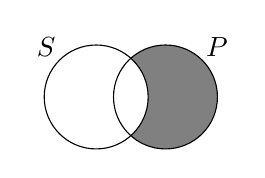
\begin{tikzpicture}
\def\firstcircle{(0,0) circle (.66cm)}
\def\secondcircle{(0:.88cm) circle (.66cm)}
     \begin{scope}[shift={(4cm,0cm)}]
        \begin{scope}[even odd rule]
            \clip \firstcircle (-.66,-.66) rectangle (1.66,.88);
        \fill[gray] \secondcircle;
        \end{scope}
        \draw \firstcircle node[outer sep=.4cm, above left] (s) {$S$};
        \draw \secondcircle node[outer sep=.4cm, above right] (p) {$P$};
    \end{scope} 
\end{tikzpicture}

\\

\textbf{A:} All $S$ are $P$

&

\textbf{A:} All $P$ are $S$

\\

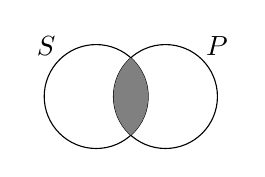
\begin{tikzpicture}
\def\firstcircle{(0,0) circle (.66cm)}
\def\secondcircle{(0:.88cm) circle (.66cm)}
\draw \firstcircle node[outer sep=.4cm, above left] (s) {$S$};
\draw \secondcircle node[outer sep=.4cm, above right] (p) {$P$};
    \begin{scope}
      \clip \firstcircle;
      \fill[gray] \secondcircle;
    \end{scope}
\end{tikzpicture}

&

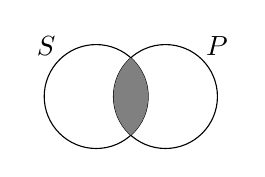
\begin{tikzpicture}
\def\firstcircle{(0,0) circle (.66cm)}
\def\secondcircle{(0:.88cm) circle (.66cm)}
\draw \firstcircle node[outer sep=.4cm, above left] (s) {$S$};
\draw \secondcircle node[outer sep=.4cm, above right] (p) {$P$};
    \begin{scope}
      \clip \firstcircle;
      \fill[gray] \secondcircle;
    \end{scope}
\end{tikzpicture}

\\

\textbf{E}: No $S$ are $P$

&
\textbf{E}: No $P$ are $S$


\\

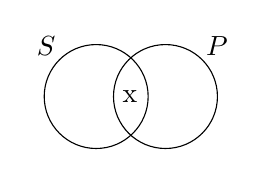
\begin{tikzpicture}
\def\firstcircle{(0,0) circle (.66cm)}
\def\secondcircle{(0:.88cm) circle (.66cm)}
\draw \firstcircle node[outer sep=.4cm, above left] (s) {$S$};
\node[outer sep=.22cm, right] (x) {x};
\draw \secondcircle node[outer sep=.4cm, above right] (p) {$P$};
\end{tikzpicture}

&

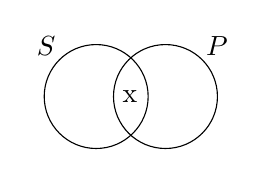
\begin{tikzpicture}
\def\firstcircle{(0,0) circle (.66cm)}
\def\secondcircle{(0:.88cm) circle (.66cm)}
\draw \firstcircle node[outer sep=.4cm, above left] (s) {$S$};
\node[outer sep=.22cm, right] (x) {x};
\draw \secondcircle node[outer sep=.4cm, above right] (p) {$P$};
\end{tikzpicture}

\\

\textbf{I}: Some $S$ are $P$

&

\textbf{I}: Some $P$ are $S$

\\

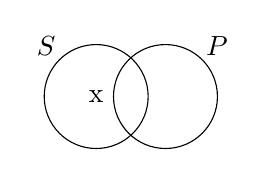
\begin{tikzpicture}
\def\firstcircle{(0,0) circle (.66cm)}
\def\secondcircle{(0:.88cm) circle (.66cm)}
\draw \firstcircle node[outer sep=.4cm, above left] (s) {$S$};
\node[outer sep=.3cm] (x) {x};
\draw \secondcircle node[outer sep=.4cm, above right] (p) {$P$};
\end{tikzpicture}

&


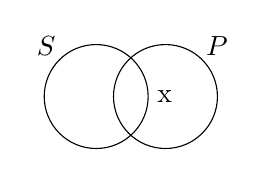
\begin{tikzpicture}
\def\firstcircle{(0,0) circle (.66cm)}
\def\secondcircle{(0:.88cm) circle (.66cm)}
\draw \firstcircle node[outer sep=.4cm, above left] (s) {$S$};
\node[outer sep=.66cm, right] (x) {x};
\draw \secondcircle node[outer sep=.4cm, above right] (p) {$P$};
\end{tikzpicture}


\\

\textbf{O}: Some $S$ are not $P$

&

\textbf{O}: Some $P$ are not $S$

\end{tabu}
\end{mdframed}
\caption{Conversions of the Four Basic Forms}
\label{fig:conversion} 	
\end{figure}

As you can see, the Venn diagram for the converse of an E statement is exactly the same as the original E statement, and likewise for I statements. This means that the two statements are logically equivalent. Recall that two statements are logically equivalent if they always have the same truth value. (See page \ref{def:logical_equivalence}). In this case, that means that if an E statement is true, then its converse is also true, and if an E statement is false, then its converse is also false. For instance, ``No dogs are reptiles'' is true, and so is ``No reptiles are dogs.'' On the other hand ``No dogs are mammals'' is false, and so is ``No mammals are dogs.''

Likewise, if an I statement is true, its converse is true, and if an I statement is false, than its converse is false. ``Some dogs are pets'' is true, and so is ``Some pets are dogs.'' On the other hand ``Some dogs can fly'' is false and so is ``Some flying things are dogs.''

The converses of A and O statements are not so illuminating. As you can see from the Venn diagrams, these statements are not identical to their converses. They also don't contradict their converses. If we know that an A or O statement is true, we still don't know anything about their converses. We say their truth value is undetermined. 

Because E and I statements are logically equivalent to their converses, we can use them to construct valid arguments. Recall from Chapter 2 (page \pageref{def:valid}) that an argument is valid if it is impossible for its conclusion to be false whenever its premises are true. Because E and I are logically equivalent to their converses, the two argument forms in Figure \ref{fig:conversion_arguments} are valid. 


\begin{figure}
\begin{mdframed}[style=mytablebox]
\begin{tabu}{p{.5\linewidth}p{.5\linewidth}}

\begin{earg}
\item[P.] No $S$ are $P$.
\vspace{-.5em}
\item [] \rule{0.6\linewidth}{1pt} 
\item[C.] No $P$ are $S$.
\end{earg} 

&

\begin{earg}
\item[P.] Some $S$ are $P$.
\vspace{-.5em}
\item [] \rule{0.6\linewidth}{1pt} 
\item[C.] Some  $P$ are $S$.
\end{earg} 
\end{tabu}
\end{mdframed}
\caption{Valid Arguments by Conversion} \label{fig:conversion_arguments}
\end{figure}

Notice that these are argument forms, with variables in the place of the key terms. This means that these arguments will be valid no matter what; $S$ and $P$ could be people, or squirrels, or the Gross Domestic Product of industrialized nations, or anything, and the arguments are still valid. While these particular argument forms may seem trivial and obvious, we are beginning to see some of the power of formal logic here. We have uncovered a very general truth about the nature of validity with these two argument forms. 

The truth value of the converses of A and O statements, on the other hand, are undetermined by the truth value of the original statements. This means we cannot construct valid arguments from them. Imagine you have an argument with an A or O statement as its premise and the converse of that statement as the conclusion. Even if the premise is true, we know nothing about the truth of the conclusion. So there are no valid argument forms to be found here. 

\subsection{Obversion}

\newglossaryentry{complement}
{
name=complement,
description={The class of everything that is not in a given class.}
}


Obversion is a more complex process. To understand what an obverse is, we first need to define the complement of a class. The \textsc{\gls{complement}} \label{def:Complement} of a class is everything that is not in the class. So the complement of the class of dogs is everything that is not a dog, including not just cats, but battleships, pop songs, and black holes. In English we can easily create a name for the complement of any class using the prefix ``non-''. So the complement of the class of dogs is the class of non-dogs. We will use complements in defining both obversion and contraposition. 

\newglossaryentry{obversion}
{
name=obversion,
description={The process of transforming a categorical statement by changing its quality and replacing the predicate with its complement.}
}


The \textsc{\gls{obversion}} \label{def:Obversion} of a categorical proposition is a new proposition created by changing the quality of the original proposition and switching its predicate to its complement. Obversion is thus a two step process. Take, again, the proposition ``All dogs are mammals.'' For step 1, we change its quality, in this case going from affirmative to negative. That gives us ``No dogs are mammals.'' For step 2, we take the complement of the predicate. The predicate in this case is ``mammals'' so the complement is ``non-mammals.'' That gives us the obverse ``No dogs are non-mammals.''

We can map this process out using Venn diagrams. Let's start with an A statement.

\begin{center}
\begin{tikzpicture}
\def\firstcircle{(0,0) circle (1cm)}
\def\secondcircle{(0:1.33cm) circle (1cm)}
     \begin{scope}[shift={(4cm,0cm)}]
        \begin{scope}[even odd rule]% first circle without the second
            \clip \secondcircle (-1,-1) rectangle (1,1);
        \fill[gray] \firstcircle;
        \end{scope}
        \draw \firstcircle node[outer sep=.75cm, above left] (s) {$S$};
        \draw \secondcircle node[outer sep=.75cm, above right] (p) {$P$};
    \end{scope}
\end{tikzpicture} \\
\textbf{A}: All $S$ are $P$.
\end{center}

Changing the quality turns it into an E statement.

\begin{center}
\begin{tikzpicture}
\def\firstcircle{(0,0) circle (1cm)}
\def\secondcircle{(0:1.33cm) circle (1cm)}
\draw \firstcircle node[outer sep=.75cm, above left] (s) {$S$};
\draw \secondcircle node[outer sep=.75cm, above right] (p) {$P$};
    \begin{scope}
      \clip \firstcircle;
      \fill[gray] \secondcircle;
    \end{scope}
\end{tikzpicture} \\
\textbf{E}: No $S$ are $P$.
\end{center}

Now what happens when we take the complement of $P$? That means we will shade in all the parts of S that are non-$P$, which puts us back where we started.


\begin{figure}[H]
\begin{center}
\begin{tikzpicture}
\def\firstcircle{(0,0) circle (1cm)}
\def\secondcircle{(0:1.33cm) circle (1cm)}
     \begin{scope}%[shift={(4cm,0cm)}]
        \begin{scope}[even odd rule]% first circle without the second
            \clip \secondcircle (-1,-1) rectangle (1,1);
        \fill[gray] \firstcircle;
        \end{scope}
        \draw \firstcircle node[outer sep=.75cm, above left] (s) {$S$};
        \draw \secondcircle node[outer sep=.75cm, above right] (p) {$P$};
    \end{scope}
\end{tikzpicture} \\
\captionsetup{singlelinecheck=on}
\caption*{\textbf{E}: No $S$ are non-$P$.}
\end{center}
\end{figure}

The final statement is logically equivalent to the original A statement. It has the same form as an E statement, but because we have changed the predicate, it is not logically equivalent to an A statement. As you can see from Figure \ref{fig:obversion} this is true for all four forms of categorical statement. 
This in turn gives us four valid argument forms, which are shown in Figure \ref{fig:obversion_arguments}

\begin{figure}
\begin{mdframed}[style=mytablebox]
\begin{tabu}{p{.5\linewidth}p{.5\linewidth}}

\underline{Original Statement}

&

\underline{Obverse} \\

\begin{tikzpicture}
\def\firstcircle{(0,0) circle (1cm)}
\def\secondcircle{(0:1.33cm) circle (1cm)}
     \begin{scope}%[shift={(4cm,0cm)}]
        \begin{scope}[even odd rule]% first circle without the second
            \clip \secondcircle (-1,-1) rectangle (1,1);
        \fill[gray] \firstcircle;
        \end{scope}
        \draw \firstcircle node[outer sep=.75cm, above left] (s) {$S$};
        \draw \secondcircle node[outer sep=.75cm, above right] (p) {$P$};
    \end{scope} 
\end{tikzpicture}

&

\begin{tikzpicture}
\def\firstcircle{(0,0) circle (1cm)}
\def\secondcircle{(0:1.33cm) circle (1cm)}
     \begin{scope}[shift={(4cm,0cm)}]
        \begin{scope}[even odd rule]% first circle without the second
            \clip \secondcircle (-1,-1) rectangle (1,1);
        \fill[gray] \firstcircle;
        \end{scope}
        \draw \firstcircle node[outer sep=.75cm, above left] (s) {$S$};
        \draw \secondcircle node[outer sep=.75cm, above right] (p) {$P$};
    \end{scope} 
\end{tikzpicture}
\\

\textbf{A:} All $S$ are $P$

&

\textbf{E:} No $S$ are non-$P$

\\

\begin{tikzpicture}
\def\firstcircle{(0,0) circle (1cm)}
\def\secondcircle{(0:1.33cm) circle (1cm)}
\draw \firstcircle node[outer sep=.75cm, above left] (s) {$S$};
\draw \secondcircle node[outer sep=.75cm, above right] (p) {$P$};
    \begin{scope}
      \clip \firstcircle;
      \fill[gray] \secondcircle;
    \end{scope}
\end{tikzpicture}

&

\begin{tikzpicture}
\def\firstcircle{(0,0) circle (1cm)}
\def\secondcircle{(0:1.33cm) circle (1cm)}
\draw \firstcircle node[outer sep=.75cm, above left] (s) {$S$};
\draw \secondcircle node[outer sep=.75cm, above right] (p) {$P$};
    \begin{scope}
      \clip \firstcircle;
      \fill[gray] \secondcircle;
    \end{scope}
\end{tikzpicture}

\\

\textbf{E}: No $S$ are $P$

&
\textbf{A}: All $S$ are non-$P$


\\

\begin{tikzpicture}
\def\firstcircle{(0,0) circle (1cm)}
\def\secondcircle{(0:1.33cm) circle (1cm)}
\draw \firstcircle node[outer sep=.75cm, above left] (S) {$S$};
\node[xshift=.66cm] (x) {X};
\draw \secondcircle node[outer sep=.75cm, above right] (P) {$P$};
\end{tikzpicture}

&

\begin{tikzpicture}
\def\firstcircle{(0,0) circle (1cm)}
\def\secondcircle{(0:1.33cm) circle (1cm)}
\draw \firstcircle node[outer sep=.75cm, above left] (s) {$S$};
\node[xshift=.66cm] (x) {X};
\draw \secondcircle node[outer sep=.75cm, above right] (p) {$P$};
\end{tikzpicture}

\\

\textbf{I}: Some $S$ are $P$

&

\textbf{O}: Some $S$ are not non-$P$

\\

\begin{tikzpicture}
\def\firstcircle{(0,0) circle (1cm)}
\def\secondcircle{(0:1.33cm) circle (1cm)}
\draw \firstcircle node[outer sep=.75cm, above left] (s) {$S$};
\node (x) {X};
\draw \secondcircle node[outer sep=.75cm, above right] (p) {$P$};
\end{tikzpicture}

&


\begin{tikzpicture}
\def\firstcircle{(0,0) circle (1cm)}
\def\secondcircle{(0:1.33cm) circle (1cm)}
\draw \firstcircle node[outer sep=.75cm, above left] (s) {$S$};
\node (x) {X};
\draw \secondcircle node[outer sep=.75cm, above right] (p) {$P$};
\end{tikzpicture}


\\

\textbf{O}: Some $S$ are not $P$

&

\textbf{I}: Some $S$ are non-$P$

\end{tabu}
\end{mdframed}
\caption{Obversions of the Four Basic Forms}
\label{fig:obversion} 	
\end{figure}



\begin{figure} %new fig
\begin{mdframed}[style=mytablebox]
\begin{tabu}{p{.5\linewidth}p{.5\linewidth}}

\begin{earg*}
\item All $S$ are $P.$
\itemc No $S$ are non-$P$.
\end{earg*} 

&

\begin{earg*}
\item No $S$ are $P$.
\itemc All $S$ are non-$P$.
\end{earg*} 

\\

\begin{earg*}
\item Some $S$ are $P$.
\itemc Some $S$ are not non-$P$.
\end{earg*} 

&

\begin{earg*}
\item Some $S$ are not $P$.
\itemc Some $S$ are non-$P$.
\end{earg*}
 
\end{tabu}
\end{mdframed}
\caption{Valid argument forms by obversion} \label{fig:obversion_arguments}
\end{figure}

One further note on complements. We don't just use complements to describe sentences that come out of obversion and contraposition. We can also perform these operations on statements that already have complements in them. Consider the sentence ``Some $S$ are non-$P$.'' This is its Venn diagram. 

\begin{figure}[H]
\begin{center}
\begin{tikzpicture}
\def\firstcircle{(0,0) circle (1cm)}
\def\secondcircle{(0:1.33cm) circle (1cm)}
\draw \firstcircle node[outer sep=.75cm, above left] (s) {$S$};
\node (x) {X};
\draw \secondcircle node[outer sep=.75cm, above right] (p) {$P$};
\end{tikzpicture}
\captionsetup{singlelinecheck=on}
\caption*{Some $S$ are non-$P$}
\end{center} 
\end{figure}

How would we take the obverse of this statement? Step 1 is to change the quality, making it ``Some $S$ are not non-$P$.'' Now how do we take the complement of the predicate? We could write ``non-non-$P$,'' but if we think about it for a second, we'd realize that this is the same thing as $P$. So we can just write ``Some $S$ is not $P$.'' This is logically equivalent to the original statement, which is what we wanted.   

Taking the converse of ``Some $S$ are non-$P$'' also takes a moment of thought. We are supposed to reverse subject and predicate. But does that mean that the ``non-'' moves to the subject position along with the ``$P$''? Or does the ``non-'' now attach to the $S$? We saw that E and I statements kept their truth value after conversion, and we want this to still be true when the statements start out referring to the complement of some class. This means that the ``non-'' has to travel with the predicate, because ``Some $S$ are non-$P$'' will always have the same truth value as ``Some non-$P$ are $S$.'' Another way of thinking about this is that the ``non-'' is part of the name of the class that forms the predicate of ``Some $S$ are non-$P$.'' The statement is making a claim about a class, and that class happens to be defined as the complement of another class. So, the bottom line is when you take the converse of a statement where one of the terms is a complement, move the ``non-'' with that term. 

\subsection{Contraposition}

\newglossaryentry{contraposition}
{
name=contraposition,
description={The process of transforming a categorical statement by reversing subject and predicate and replacing them with their complements.}
}


\textsc{\gls{contraposition}} is a two-step process, like obversion, but it doesn't always lead to results that are logically equivalent to the original sentence. The contrapositive of a categorical sentence is the sentence that results from reversing subject and predicate and then replacing them with their complements. Thus ``All $S$ are $P$'' becomes ``All non-$P$ are non-$S$.'' 

Figure \ref{fig:contraposition} shows the corresponding Venn diagrams. In this case, the shading around the outside of the two circles in the contraposed form of E is meant to indicate that nothing can lie outside the two circles. Everything must be $S$ or $P$ or both. Like conversion, applying contraposition to two of the forms gives us statements that are logically equivalent to the original. This time, though, it is forms A and O that come through the process without changing their truth value. 

\begin{figure}
\begin{mdframed}[style=mytablebox]
\begin{tabu}{p{.5\linewidth}p{.5\linewidth}}

\underline{Original Statement}

&

\underline{Contrapositive} \\

\begin{tikzpicture}
\def\firstcircle{(0,0) circle (.66cm)}
\def\secondcircle{(0:.88cm) circle (.66cm)}
     \begin{scope}[shift={(4cm,0cm)}]
        \begin{scope}[even odd rule]% first circle without the second
            \clip \secondcircle (-.66,-.66) rectangle (.66,.66);
        \fill[gray] \firstcircle;
        \end{scope}
        \draw \firstcircle node[outer sep=.4cm, above left] (s) {$S$};
        \draw \secondcircle node[outer sep=.4cm, above right] (p) {$P$};
    \end{scope} 
\end{tikzpicture}

&

\begin{tikzpicture}
\def\firstcircle{(0,0) circle (.66cm)}
\def\secondcircle{(0:.88cm) circle (.66cm)}
     \begin{scope}[shift={(4cm,0cm)}]
        \begin{scope}[even odd rule]% first circle without the second
            \clip \secondcircle (-.66,-.66) rectangle (.66,.66);
        \fill[gray] \firstcircle;
        \end{scope}
        \draw \firstcircle node[outer sep=.4cm, above left] (s) {$S$};
        \draw \secondcircle node[outer sep=.4cm, above right] (p) {$P$};
    \end{scope} 
\end{tikzpicture}
\\

\textbf{A:} All $S$ are $P$

&

\textbf{A:} All non-$P$ are non-$S$

\\

\begin{tikzpicture}
\def\firstcircle{(0,0) circle (.66cm)}
\def\secondcircle{(0:.88cm) circle (.66cm)}
\draw \firstcircle node[outer sep=.4cm, above left] (s) {$S$};
\draw \secondcircle node[outer sep=.4cm, above right] (p) {$P$};
    \begin{scope}
      \clip \firstcircle;
      \fill[gray] \secondcircle;
    \end{scope}
\end{tikzpicture}

&

\begin{tikzpicture}
\def\firstcircle{(0,0) circle (.66cm)}
\def\secondcircle{(0:.88cm) circle (.66cm)}

\fill[gray] (-.88,-.88) rectangle (1.88,.88);
\fill[light-gray] 
    \firstcircle node[outer sep=.4cm, above left] (s) {$S$}
    \secondcircle node[outer sep=.4cm, above right] (p) {$P$};
\draw
    \firstcircle 
    \secondcircle ;
\end{tikzpicture}
\\

\textbf{E}: No $S$ are $P$

&
\textbf{E}: No non-$P$ are non-$S$


\\

\begin{tikzpicture}
\def\firstcircle{(0,0) circle (.66cm)}
\def\secondcircle{(0:.88cm) circle (.66cm)}
\draw \firstcircle node[outer sep=.4cm, above left] (s) {$S$};
\node[outer sep=.22cm, right] (x) {x};
\draw \secondcircle node[outer sep=.4cm, above right] (p) {$P$};
\end{tikzpicture}

&

\begin{tikzpicture}
\def\firstcircle{(0,0) circle (.66cm)}
\def\secondcircle{(0:.88cm) circle (.66cm)}
\draw \firstcircle node[outer sep=.4cm, above left] (s) {$S$};
\node[outer sep=2cm, right] (x) {x};
\draw \secondcircle node[outer sep=.4cm, above right] (p) {$P$};
\end{tikzpicture}

\\

\textbf{I}: Some $S$ are $P$

&

\textbf{I}: Some non-$P$ are non-$S$

\\

\begin{tikzpicture}
\def\firstcircle{(0,0) circle (.66cm)}
\def\secondcircle{(0:.88cm) circle (.66cm)}
\draw \firstcircle node[outer sep=.4cm, above left] (s) {$S$};
\node[outer sep=.3cm] (x) {x};
\draw \secondcircle node[outer sep=.4cm, above right] (p) {$P$};
\end{tikzpicture}

&


\begin{tikzpicture}
\def\firstcircle{(0,0) circle (.66cm)}
\def\secondcircle{(0:.88cm) circle (.66cm)}
\draw \firstcircle node[outer sep=.4cm, above left] (s) {$S$};
\node[outer sep=.3cm] (x) {x};
\draw \secondcircle node[outer sep=.4cm, above right] (p) {$P$};
\end{tikzpicture}


\\

\textbf{O}: Some $S$ are not $P$

&

\textbf{O}: Some non-$P$ are not non-$S$

\end{tabu}
\end{mdframed}
\caption{Contrapositions the Four Basic Forms}
\label{fig:contraposition} 	
\end{figure}

This then gives us two valid argument forms, shown in Figure \ref{fig:argument_contraposition}. If you have an argument with an A or O statement as its premise and the contraposition of that statement as the conclusion, you know it must be valid. Whenever the premise is true, the conclusion must be true, because the two statements are logically equivalent. On the other hand, if you had an E or an I statement as the premise, the truth of the conclusion is undetermined, so these arguments would not be valid. 


\begin{figure}
\begin{mdframed}[style=mytablebox]
\begin{tabu}{p{.5\linewidth}p{.5\linewidth}}

\begin{earg*}
\item All $S$ are $P$.
\itemc All non-$P$ are non-$S$.
\end{earg*} 


&


\begin{earg*}
\item Some $S$ are not $P$
\itemc Some non-$P$ are not non-$S$.
\end{earg*}

\end{tabu}
\end{mdframed}
\caption{Valid argument forms from contraposition} \label{fig:argument_contraposition}
\end{figure}

\subsection{Evaluating Short Arguments}
\label{sec:ESA}
So far we have seen eight valid forms of argument with one premise: two arguments that are valid by conversion, four that are valid by obversion, and two that are valid by contraposition. As we said, short arguments like these are sometimes called ``immediate inferences,'' because your brain just flits automatically from the truth of the premises to the truth of the conclusion. Now that we have identified these valid forms of inference, we can use this knowledge to see whether some of the arguments we encounter in ordinary language are valid. We can now tell in a few cases if our brain is right to flit so seamlessly from the premise to the conclusion.

In the real world, the inferences we make are messy and hard to classify. Much of the complexity of this issue is tackled in the parts of the complete version of this text that cover critical thinking. \label{ver_var} \nix{Part \ref{part:CT_and_informal_logic} of this text, on critical thinking.} Right now we are just going to deal with a limited subset of inferences: immediate inferences that might be based on conversion, obversion, or contraposition. Let's start start with the uncontroversial premise ``All dogs are mammals.'' Can we infer from this that all non-mammals are non-dogs? In canonical form, the argument would look like this. 

\pagebreak[4] %Note the hard page break. Delete if things start to drift.

\begin{earg*}
\item All dogs are mammals
\itemc[.3] All non-mammals are non-dogs.
\end{earg*} 

Evaluating an immediate inference like this is a four step process. First, identify the subject and predicate classes. Second, draw the Venn diagram for the premise. Third, see if the Venn diagram shows that the conclusion must be true. If it must be, then the argument is valid. Finally, if the argument is valid, identify the process that makes it valid. (You can skip this step if the argument is invalid.)

For the argument above, the result of the first two steps would look like this:   

\begin{figure}[H]
\begin{center}
\begin{tikzpicture}
\def\firstcircle{(0,0) circle (.66cm)}
\def\secondcircle{(0:.88cm) circle (.66cm)}
     \begin{scope}[shift={(4cm,0cm)}]
        \begin{scope}[even odd rule]% first circle without the second
            \clip \secondcircle (-.66,-.66) rectangle (.66,.66);
        \fill[gray] \firstcircle;
        \end{scope}
        \draw \firstcircle node[outer sep=.4cm, above left] (s) {$S$};
        \draw \secondcircle node[outer sep=.4cm, above right] (p) {$P$};
    \end{scope} 
\end{tikzpicture}
\end{center}
\captionsetup{singlelinecheck=on}
\caption*{$S$: Dogs \\ $P$: Mammals}
\end{figure}

The Venn diagram for the premise shades out the possibility that there are dogs that aren't mammals. For step three, we ask, does this mean the conclusion must be true?  In this case, it does. The same shading implies that everything that is not a mammal must also not be a dog. In fact, the Venn diagram for the premise and the Venn diagram for the conclusion are the same. So the argument is valid. This means that we must go on to step four and identify the process that makes it valid. In this case, the conclusion is created by reversing subject and predicate and taking their complements, which means that this is a valid argument by contraposition.
   
Now, remember what it means for an argument to be valid. \label{valid_definition_reinforcement} As we said on page \pageref{def:valid}, an argument is valid if it is impossible for the premises to be true and the conclusion false. This means that we can have a valid argument with false premises, so long as it is the case that \emph{if} the premises were true, the conclusion would have to be true. So if the argument above is valid, then so is this one:

\begin{earg*}
\item All dogs are reptiles.
\itemc[.3] All non-reptiles are non-dogs.
\end{earg*}

The premise is now false: all dogs are not reptiles. However, \emph{if} all dogs were reptiles, then it would also have to be true that all non-reptiles are non-dogs. The Venn diagram works the same way.

\begin{figure}[H]
\begin{center}
\begin{tikzpicture}
\def\firstcircle{(0,0) circle (.66cm)}
\def\secondcircle{(0:.88cm) circle (.66cm)}
     \begin{scope}[shift={(4cm,0cm)}]
        \begin{scope}[even odd rule]% first circle without the second
            \clip \secondcircle (-.66,-.66) rectangle (.66,.66);
        \fill[gray] \firstcircle;
        \end{scope}
        \draw \firstcircle node[outer sep=.4cm, above left] (s) {$S$};
        \draw \secondcircle node[outer sep=.4cm, above right] (p) {$P$};
    \end{scope} 
\end{tikzpicture}
\end{center}
\captionsetup{singlelinecheck=on}
\caption*{$S$: Dogs \\ $P$: Reptiles}
\end{figure}

The Venn diagram for the premise still matches the Venn diagram for the conclusion. Only the labels have changed. The fact that this argument form remains true even with a false premise is just a variation on a theme we saw in 
Figure \ref{fig:valid_sound} when we saw a valid argument (with false premises) for the conclusion ``Socrates is a carrot.'' So arguments by transposition, just like any argument, can be valid even if they have false premises. The same is true for arguments by conversion and obversion. 

Arguments like these can also be invalid, even if they have true premises and a true conclusion. Remember that A statements are not logically equivalent to their converse. So this is an invalid argument with a true premise and a false conclusion:

\begin{earg*}
\item All dogs are mammals.
\itemc[.3] All mammals are dogs. 
\end{earg*}

Our Venn diagram test shows that this is invalid. Steps one and two give us this for the premise:
\begin{figure}[H]
\begin{center}
\begin{tikzpicture}
\def\firstcircle{(0,0) circle (.66cm)}
\def\secondcircle{(0:.88cm) circle (.66cm)}
     \begin{scope}[shift={(4cm,0cm)}]
        \begin{scope}[even odd rule]% first circle without the second
            \clip \secondcircle (-.66,-.66) rectangle (.66,.66);
        \fill[gray] \firstcircle;
        \end{scope}
        \draw \firstcircle node[outer sep=.4cm, above left] (s) {$S$};
        \draw \secondcircle node[outer sep=.4cm, above right] (p) {$P$};
    \end{scope} 
\end{tikzpicture}
\end{center}
\captionsetup{singlelinecheck=on}
\caption*{$S$: Dogs \\ $P$: Mammals}
\end{figure}

But this is the Venn diagram for the conclusion:

\begin{figure}[H]
\begin{center}
\begin{tikzpicture}
\def\firstcircle{(0,0) circle (.66cm)}
\def\secondcircle{(0:.88cm) circle (.66cm)}
     \begin{scope}[shift={(4cm,0cm)}]
        \begin{scope}[even odd rule]% first circle without the second
            \clip \firstcircle (-.66,-.66) rectangle (1.66,.88);
        \fill[gray] \secondcircle;
        \end{scope}
        \draw \firstcircle node[outer sep=.4cm, above left] (s) {$S$};
        \draw \secondcircle node[outer sep=.4cm, above right] (p) {$P$};
    \end{scope} 
\end{tikzpicture}
\end{center}
\captionsetup{singlelinecheck=on}
\caption*{$S$: Dogs \\ $P$: Mammals}
\end{figure}

This is an argument by conversion on an mood-A statement, which is invalid. The argument remains invalid, even if we substitute in a predicate where the conclusion happens to be true. For instance this argument is invalid.

\begin{earg*}
\item  All dogs are \textit{Canis familiaris}.
\itemc[.4] All \textit{Canis familiaris} are dogs. 
\end{earg*}

The Venn diagrams for the premise and conclusion of this argument will be just like the ones for the previous argument, just with different labels. So even though the argument has a true premise and a true conclusion, it is still invalid, because it is possible for an argument of this form to have a true premise and a false conclusion. This is an unreliable argument form that just happened, in this instance, not to lead to a false conclusion. This again is just a variation on a theme we saw in Chapter \ref{chap:basicevaluation}, in Figure \ref{fig:invalid_paris}, when we saw an invalid argument for the conclusion that Paris was in France.


%%%%%%%%%%%%%%%%%%%%% practice problems %%%%%%%%%%%%%

\practiceproblems
\problempart The first two columns in the table below give you a statement and a truth value for that statement. The next column gives an operation that can be performed on the statement in the first column, and the final two columns give the new statement and its truth value. 

The first row is completed, as an example, but after that there are blanks. In problems 1--5 you must fill in the new statement and its truth value, and in problems 6--10 you must fill in the operation and the final truth value. If the truth value of the resulting statement cannot be determined from the original one, write a ``?'' for ``undetermined.'' You can check your work with Venn diagrams, or by identifying the logical form of the original statement and seeing if it is one where the named operation changes the truth value. 

\begin{longtabu}{X[1,l,m]X[15,l,m]X[2,l,m]X[6,l,m]X[16,l,m]X[1,l,m]}
%{p{.01\linewidth}p{.2\linewidth}p{.15\linewidth}p{.15\linewidth}p{.2\linewidth}p{.1\linewidth}}
%{llllll} 
 & \underline{Given statement} & \underline{T/F} & \underline{Operation} & \underline{New Statement} & \underline{T/F} \\
  \rowcolor{light-gray}
 Ex. & All $S$ are $P$ & F & Conv. & All $P$ are $S$ & ? \\ 
 \endhead
 
1. & Some $S$ are $P$  & F  & Obv. & \answerblank{Some $S$ are not non-$P$}{\rule[-5pt]{2.5cm}{.4pt}}& \answerblank{F}{\rule[-5pt]{.5cm}{.4pt}}\\



2.& Some non-$S$ are $P$  & F& Conv. & \answerblank{Some $P$ are non-$S$}{\rule[-5pt]{2.5cm}{.4pt}}&\answerblank{F}{\rule[-5pt]{.5cm}{.4pt}}\\


3. & All $S$ are $P$  & F & Contrap. & \answerblank{All non-$P$ are non-$S$}{\rule[-5pt]{2.5cm}{.4pt}}& \answerblank{F}{\rule[-5pt]{.5cm}{.4pt}}\\

4. & Some $S$ are $P$  & F & Contrap. & \answerblank{Some non-$P$ are non-$S$}{\rule[-5pt]{2.5cm}{.4pt}}& \answerblank{?}{\rule[-5pt]{.5cm}{.4pt}}\\

5. & Some $S$ are non-$P$ & T & Obv. & \answerblank{Some $S$ are not $P$}{\rule[-5pt]{2.5cm}{.4pt}}& \answerblank{T}{\rule[-5pt]{.5cm}{.4pt}}\\

6.& All $S$ are non-$P$  & T & \answerblank{Contrap.}{\rule[-5pt]{1.5cm}{.4pt}}& All $P$ are non-$S$ & \answerblank{T}{\rule[-5pt]{.5cm}{.4pt}}\\

7.& Some non-$S$ are not P & T & \answerblank{Conv.}{\rule[-5pt]{1.5cm}{.4pt}}& Some $P$ are not non-$S$ & \answerblank{?}{\rule[-5pt]{.5cm}{.4pt}}\\

8. & Some $S$ are not P & F  & \answerblank{Conv.}{\rule[-5pt]{1.5cm}{.4pt}}& Some $P$ are not $S$ & \answerblank{?}{\rule[-5pt]{.5cm}{.4pt}}\\

9.& All non-$S$ are $P$ & T & \answerblank{Obv.}{\rule[-5pt]{1.5cm}{.4pt}}& No non-$S$ are non-$P$ & \answerblank{T}{\rule[-5pt]{.5cm}{.4pt}}\\

10. & No non-$S$ are non-$P$ & T & \answerblank{Obv.}{\rule[-5pt]{1.5cm}{.4pt}} & All non-$S$ are non-non-$P$ & \answerblank{T}{\rule[-5pt]{.5cm}{.4pt}}\\ 
  
\end{longtabu}

\problempart See the instructions for Part A.

\begin{longtabu}{X[1,l,m]X[15,l,m]X[2,l,m]X[6,l,m]X[16,l,m]X[1,l,m]}
%{p{.01\linewidth}p{.2\linewidth}p{.15\linewidth}p{.15\linewidth}p{.2\linewidth}p{.1\linewidth}}
%{llllll} 
 & \underline{Given statement} & \underline{T/F} & \underline{Operation} & \underline{New Statement} & \underline{T/F} \\

  

1. & All $S$ are $P$& T & Obv. & \nix{ } \rule[-5pt]{2.5cm}{.4pt}  & \nix{ } \rule[-5pt]{.5cm}{.4pt} \\ 

2.& Some $S$ are not non-$P$& T & Contrap. & \nix{ } \rule[-5pt]{2.5cm}{.4pt} &\nix{ } \rule[-5pt]{.5cm}{.4pt} \\


3. & No $S$ are non-$P$& T & Obv. & \nix{  } \rule[-5pt]{2.5cm}{.4pt} & \nix{ } \rule[-5pt]{.5cm}{.4pt} \\

4. & All non-$S$ are $P$& T & Obv. & \nix{ } \rule[-5pt]{2.5cm}{.4pt}& \nix{ } \rule[-5pt]{.5cm}{.4pt} \\

5. & Some non-$S$ are $P$& F & Contrap. & \nix{ } \rule[-5pt]{2.5cm}{.4pt}& \nix{ } \rule[-5pt]{.5cm}{.4pt} \\

6. & Some $S$ are $P$& F &  \nix{Obv.} \rule[-5pt]{1.5cm}{.4pt} & Some $S$ are not non-$P$  & \nix{F} \rule[-5pt]{.5cm}{.4pt} \\ 

7.& No non-$S$ are non-$P$& F &  \nix{Contrap.} \rule[-5pt]{1.5cm}{.4pt} & No $P$ are $S$  & \nix{?}\rule[-5pt]{.5cm}{.4pt} \\

8. & Some non-$S$ are non-$P$& T & \nix{Contrap.} \rule[-5pt]{1.5cm}{.4pt} & Some $P$ are $S$ & \nix{?} \rule[-5pt]{.5cm}{.4pt} \\

9.& All $S$ are $P$ & F & \nix{Obv.}\rule[-5pt]{1.5cm}{.4pt}  & No $S$ are non-$P$  & \nix{F} \rule[-5pt]{.5cm}{.4pt} \\

10. &  Some non-$S$ are not non-$P$ &  T & \nix{Obv.} \rule[-5pt]{1.5cm}{.4pt}  &Some non-$S$ are $P$   & \nix{T}  \rule[-5pt]{.5cm}{.4pt} \\
 \end{longtabu}

\noindent \problempart For each sentence, write the converse, obvserse, or contrapostive as directed.

\begin{longtabu}{p{.1\linewidth}p{.9\linewidth}}
\textbf{Example}: & Write the contrapositive of ``Some sentences are categorical.''\\
\textbf{Answer}: & Some non-categorical things are non-sentences. \\
\end{longtabu}

\begin{exercises}
\item Write the converse of ``No weeds are benign.''
\answer{\\No benign things are weeds}
 
\item Write the converse of ``Some minds are not closed.'' 
\answer{\\Some closed things are not minds}

\item Write the contraposition of ``Some dentists are underpaid.'' 
\answer{\\Some non-underpaid people are non-dentists}

\item Write the converse of ``All humor is good.'' 
\answer{\\All good things are humorous}

\item Write the contraposition of ``No organizations are self-sustaining.'' 
\answer{\\No non-self-sustaining things are non-organizations} 

\item Write the obverse of ``Some dogs have fleas.'' 
\answer{\\Some dogs are not non-flea-havers. \\
or Some dogs are not non-flea-having things.}

\item Write the converse of ``Some things that have fleas are dogs.'' 
\answer{\\Some dogs have fleas}

\item Write the obverse of ``No detectives are uniformed.'' 
\answer{\\All detectives are ununiformed. }

\item Write the converse of ``No monkeys are well-behaved.'' 
\answer{\\No well-behaved things are monkeys"}

\item Write the contraposition of ``No donkeys are obedient.'' 
\answer{\\No disobedient things are non-donkeys." }

\end{exercises}

\noindent \problempart For each sentence, write the converse, obvserse, or contrapostive as directed.
\begin{exercises} 
\item Write the converse of ``No supplies are limited.'' 
\item Write the obverse of ``No knives are toys.'' 
\item Write the contraposition of ``All logicians are rational.'' 
\item Write the obverse of ``All uniforms are clothing.'' 
\item Write the converse of ``All risks are negligible.'' 
\item Write the contraposition of ``No bestsellers are great works of literature.'' 
\item Write the obverse of ``Some descriptions are accurate.'' 
\item Write the contraposition of ``Some ties are not tacky.'' 
\item Write the obverse of ``All spies are concealed.'' 
\item Write the contraposition of ``No valleys are barren.'' 
\end{exercises}

\noindent \problempart Determine whether the following arguments are valid by drawing a Venn diagram for the premise. If they are valid, say whether they are valid by conversion, obversion, or contraposition.

\begin{longtabu}{p{.2\linewidth}p{.8\linewidth}}
\textbf{Example 1}: & All swans are white. Therefore, no swans are non-white.\\
\textbf{Answer}: & \\
&\noindent \begin{tikzpicture}
\def\firstcircle{(0,0) circle (.75cm)}
\def\secondcircle{(0:1cm) circle (.75cm)}
     \begin{scope}[shift={(4cm,0cm)}]
        \begin{scope}[even odd rule]% first circle without the second
            \clip \secondcircle (-1,-1) rectangle (1,1);
        \fill[gray] \firstcircle;
        \end{scope}
\draw \firstcircle node[outer sep=.66cm, above left] (s) {$S$};
\draw \secondcircle node[outer sep=.66cm, above right] (p) {$P$};
        \end{scope}
\end{tikzpicture}\\
& $S$: Swans \\
&$P$: White things. \\
& Valid, because the Venn diagram for the premise also makes the conclusion true.\\
& Obversion.\\
\end{longtabu}

\begin{longtabu}{p{.2\linewidth}p{.8\linewidth}}
\textbf{Example 2}: & Some dogs are pets. Therefore, some non-pets are non-dogs. \\
\textbf{Answer}: & \\
&\noindent \begin{tikzpicture}
\def\firstcircle{(0,0) circle (.75cm)}
\def\secondcircle{(0:1cm) circle (.75cm)}
     \begin{scope}[shift={(4cm,0cm)}]
        \begin{scope}[even odd rule]% first circle without the second
            \clip \secondcircle (-1,-1) rectangle (1,1);
        \fill[gray] \firstcircle;
        \end{scope}
\draw \firstcircle node[outer sep=.66cm, above left] (s) {$S$};
\draw \secondcircle node[outer sep=.66cm, above right] (p) {$P$};
        \end{scope}
\end{tikzpicture}\\
& $S$: Pets\\
&$P$: Dogs. \\
& Invalid, because the Venn diagram for the premise doesn't make the conclusion true.\\
\end{longtabu}

\begin{exercises}
\item Some smurfs are not blue. Therefore, some blue things are not smurfs.

\answer{
\begin{venns}
\someexistonesent
\drawsubsent
\drawpredsent
\end{venns}\\

S: Smurfs \\
P: Blue things\\
Invalid, because the Venn diagram for the premise does not make the conclusion true. }

\item All giraffes are majestic. Therefore, all non-majestic things are non-giraffes. 

\answer{
\begin{venns}
%\someexistonesent
\shadecomplementred{\subjectcircle}{\subjectsquare}{\predicatecircle}
\drawsubsent
\drawpredsent
\end{venns}\\
S: Giraffes\\
P: Majestic things\\
Valid, because the diagram for the premise is also the diagram for the conclusion.\\
Contraposition on a mood-A statement

}


\item Some roosters are not pets.	Therefore, some pets are not roosters.  

\answer{
\begin{venns}
\someexistonesent
%\shadecomplementred{\subjectcircle}{\subjectsquare}{\predicatecircle}
\drawsubsent
\drawpredsent
\end{venns}\\
S: Pets\\
P: Roosters\\
%Valid, because the diagram for the premise is also the diagram for the conclusion.
Invalid, because the Venn diagram for the premise does not make the conclusion true.
 }

\item No anesthesiologists are doctors. Therefore, no doctors are anesthesiologists.  

\answer{
\begin{venns}
%\someexistonesent
%\shadecomplementred{\subjectcircle}{\subjectsquare}{\predicatecircle}
\shadeintersectred{\subjectcircle}{\predicatecircle}
\drawsubsent
\drawpredsent
\end{venns}\\
S: Anesthesiologists\\
P: Soctors\\
Valid, because the diagram for the premise is also the diagram for the conclusion.
%Invalid, because the Venn diagram for the premise does not make the conclusion true.
Conversion on a mood-E statement. 
}

\item All penguins are flightless. Therefore, all flightless things are penguins. 

\answer{
\begin{venns}
%\someexistonesent
\shadecomplementred{\subjectcircle}{\subjectsquare}{\predicatecircle}
%\shadeintersectred{\subjectcircle}{\predicatecircle}
\drawsubsent
\drawpredsent
\end{venns}\\
S: Penguins\\
P: Flightless things \\
%Valid, because the diagram for the premise is also the diagram for the conclusion.
Invalid, because the Venn diagram for the premise does not make the conclusion true.
%Conversion.
}

\item No kisses are innocent. Therefore, no non-innocent things are non-kisses. 

\answer{
\begin{venns}
%\someexistonesent
%\shadecomplementred{\subjectcircle}{\subjectsquare}{\predicatecircle}
\shadeintersectred{\subjectcircle}{\predicatecircle}
\drawsubsent
\drawpredsent
\end{venns}\\
S: Kisses\\
P: Innocent things\\

%Invalid, because the Venn diagram for the premise does not make the conclusion true. 
Contraposition on a mood-E statement. 
}

\item All operas are sung. Therefore, all sung things are operas.

\answer{
\begin{venns}
%\someexistonesent
\shadecomplementred{\subjectcircle}{\subjectsquare}{\predicatecircle}
%\shadeintersectred{\subjectcircle}{\predicatecircle}
\drawsubsent
\drawpredsent
\end{venns}\\
S: Operas \\
P: Things that are sung\\
%Valid, because the diagram for the premise is also the diagram for the conclusion.
Invalid, because the Venn diagram for the premise does not make the conclusion true.
}
\item Some shopping malls are not abandoned. Therefore, some shopping malls are non-abandoned.    
\answer{
\begin{venns}
\someexistonesent
%\shadecomplementred{\subjectcircle}{\subjectsquare}{\predicatecircle}
%\shadeintersectred{\subjectcircle}{\predicatecircle}
\drawsubsent
\drawpredsent
\end{venns}\\
S: \\
P: \\
Valid, because the diagram for the premise is also the diagram for the conclusion.\\
%Invalid, because the Venn diagram for the premise does not make the conclusion true.
Obversion--always valid}

\item Some great-grandfathers are not deceased. Therefore, some non-deceased people are not non-great-grandfathers. 

\answer{
\begin{venns}
\someexistonesent
\drawsubsent
\drawpredsent
\end{venns}\\
S: Great-grandfathers\\
P: Deceased people\\
Valid, because the diagram for the premise is also the diagram for the conclusion. \\
%Invalid, because the Venn diagram for the premise does not make the conclusion true.
Contraposition on an O statement. 
}

\item Some boats are not seaworthy. Therefore, some boats are non-seaworthy.

\answer{
\begin{venns}
\someexistonesent
%\shadecomplementred{\subjectcircle}{\subjectsquare}{\predicatecircle}
%\shadeintersectred{\subjectcircle}{\predicatecircle}
\drawsubsent
\drawpredsent
\end{venns}\\
S: Boats\\
P: Seaworthy things\\
Valid, because the diagram for the premise is also the diagram for the conclusion.\\
%Invalid, because the Venn diagram for the premise does not make the conclusion true.
Obversion--always valid. 
}
\end{exercises}


\noindent \problempart Determine whether the following arguments are valid by drawing a Venn diagram for the premise. If they are valid, say whether they are valid by conversion, obversion, or contraposition.

\begin{exercises}
\item No platypuses are spies. Therefore, no non-platypuses are non-spies.     
\item All sunburns are painful. Therefore, all painful things are sunburns. 
\item All ghosts are friendly. Therefore, all non-friendly things are non-ghosts.  
\item Some philosophers are not logicians. Therefore, some philosophers are non-logicians. 
\item Some felines are lions. Therefore, some felines are not non-lions.  
\item No doubts are unreasonable. Therefore, no reasonable things are non-doubts.      
\item All Mondays are weekdays. Therefore, no Mondays are non-weekdays.  
\item Some colors are pastels. Therefore, some pastel things are colors.  
\item All dogs are cosmonauts. Therefore, all cosmonauts are dogs.     
\item All cobwebs are made of spider silk. 	Therefore, no cobwebs are made of non-spider silk.  
\end{exercises}

% ***********************************
% * The Traditional Square of Opposition *
% ***********************************

\section{The Traditional Square of Opposition}

We have seen that conversion, obversion, and contraposition allow us to identify some valid one-premise arguments. There are actually more we can find out there, but investigating them is a bit more complicated. The original investigation made by the Aristotelian philosophers made an assumption that logicians no longer make.  To help you understand all sides of the issue, we will begin by looking at things in the traditional Aristotelian fashion, and then in the next section move on to the modern way of looking at things. 

When Aristotle was first investigating these four kinds of categorical statements, he noticed they they conflicted with each other in different ways. If you are just thinking casually about it, you might say that ``No $S$ is $P$'' is somehow ``the opposite'' of ``All $S$ is $P$.'' But isn't the real ``opposite'' of ``All $S$ is $P$'' actually ``Some $S$ is not $P$''?  

Aristotle, in his book \textit{On Interpretation} (c. 350 \textsc{bce}/1\citeyear{Aristotle1984a}), notes that the real opposite of A is O, because one must always be true and the other false.  If we know that ``All dogs are mammals'' is true, then we know ``some dog is not a mammal'' is false. On the other hand, if ``All dogs are mammals'' is false then ``some dog is not a mammal'' must be true. Back on page \pageref{def:contradictory} we said that when two propositions must have opposite truth values they are called contradictories. Aristotle noted that A and O sentences are contradictory in this way. Forms E and I also form a contradictory pair. If ``Some dogs are mammals'' then ``No dogs are mammals'' is false, and if ``Some dogs are mammals'' is false, then ``No dogs are mammals'' is true.


\newglossaryentry{contraries}
{
name=contraries,
description={Two statements that can't both be true, but can both be false. A set two inconsistent sentences.}
}


Mood-A and mood-E statements are opposed to each other in a different way. Aristotle claimed that they can't both be true, but could both be false. Take the statements ``All dogs are strays'' and ``No dogs are strays.'' We know that they are both false, because some dogs are strays and others aren't. However, it is also clear that they could not both be true. When a pair of statements cannot both be true, but might both be false, the Aristotelian tradition says they are \textsc{\gls{contraries}}. \label{def:Contraries} Aristotle's idea of a pair of contraries is really just a specific case of a set of sentences that are \emph{inconsistent}, an idea that we looked at in Chapter \ref{chap:whatisformallogic}. (See page \ref{def:inconsistency})

\newglossaryentry{square of opposition}
{
name=square of opposition,
description={A way of representing the four basic propositions and the ways they relate to one another.}
}


These distinctions, plus a few other comments from Aristotle, were developed by his later followers into an idea that came to be known as the \textsc{\gls{square of opposition}} \label{def:Squareofopposition}. The square of opposition is simply the diagram you see in Figure \ref{fig:traditionalsquare}. It is a way of representing the four basic propositions and the ways they relate to one another.  As we said before, this way of picturing the proposition turned out to make a problematic assumption. To emphasize that this is no longer the way logicians view things, we will call this diagram the traditional square of opposition. 

\begin{figure}
\begin{mdframed}[style=mytablebox]
\begin{center}
\begin{tikzpicture}

\node[{font=\fontsize{45}{45}\selectfont\sf}, draw, regular polygon,regular polygon sides=8] (A) at (-4, 4) {A};
	\node [gray, xshift=-.75em, yshift=-.75em] (A-Under-True) at (A.south) {\large{T}}; 
	\node[gray, xshift=.75em, yshift=-.75em](A-Under-False) at (A.south) {\large{F}};
	\node[gray, xshift=.75em, yshift=.75em](A-Right-True) at (A.east) {\large{T}};
	\node[gray, xshift=.75em, yshift=-.6em](A-Right-False) at (A.east) {\large{F}};
	\node[gray, yshift=-1em, xshift=.2em](A-Corner-True) at (A.south east) {\large{T}};
	\node[gray, xshift=1em, yshift=-.2em](A-Corner-False) at (A.south east) {\large{F}};

\node[{font=\fontsize{45}{45}\selectfont\sf}, draw, regular polygon,regular polygon sides=8] (E) at ( 4, 4) {E};
	\node [xshift=-.75em, yshift=-.75em, gray] (E-Under-True) at (E.south) {\large{T}}; 
	\node[xshift=.75em, yshift=-.75em, gray](E-Under-False) at (E.south) {\large{F}};
	\node [xshift=-.75em, yshift=-.6em, gray] (E-Left-True) at (E.west) {\large{T}}; 
	\node[xshift=-.75em, yshift=.75em, gray](E-Left-False) at (E.west) {\large{F}};
	\node[gray, yshift=-1em, xshift=-.2em](E-Corner-True) at (E.south west) {\large{T}};
	\node[gray, xshift=-1em, yshift=-.2em](E-Corner-False) at (E.south west) {\large{F}};
\node[{font=\fontsize{45}{45}\selectfont\sf}, draw, regular polygon,regular polygon sides=8] (O) at ( 4, -4){O};
	\node [yshift=.75em, xshift=-.75em, gray] (O-Over-True) at (O.north) {\large{T}}; 
	\node[yshift=.75em, xshift=.75em, gray](O-Over-False) at (O.north) {\large{F}};
	\node [yshift=-.75em, xshift=-.75em, gray] (O-Left-True) at (O.west) {\large{T}}; 
	\node[yshift=.6em, xshift=-.75em, gray](O-Left-False) at (O.west) {\large{F}};
	\node[gray, yshift=1em, xshift=-.2em](O-Corner-True) at (O.north west) {\large{T}};
	\node[gray, xshift=-1em, yshift=.2em](O-Corner-False) at (O.north west) {\large{F}};

\node[{font=\fontsize{45}{45}\selectfont\sf}, draw, regular polygon,regular polygon sides=8] (I) at (-4,-4) {I};
	\node [yshift=.75em, xshift=-.75em, gray] (I-Over-True) at (I.north) {\large{T}}; 
	\node[yshift=.75em, xshift=.75em, gray](I-Over-False) at (I.north) {\large{F}};
	\node[yshift=.6em, xshift=.75em, gray](I-Right-True) at (I.east) {\large{T}};
	\node[yshift=-.75em, xshift=.75em, gray](I-Right-False) at (I.east) {\large{F}};
	\node[gray, yshift=1em, xshift=.2em](I-Corner-True) at (I.north east) {\large{T}};
	\node[gray, xshift=1em, yshift=.2em](I-Corner-False) at (I.north east) {\large{F}};

\draw [myarrow1] (A-Under-True) to node [xshift=-2.25em, rotate=90] {\color{black} Subalternation} node[xshift=-1em, rotate=90] {\color{gray}False up, true down}(I-Over-True); 
\draw [myarrow1] (I-Over-False) to (A-Under-False); 
\draw [myarrow1] (E-Under-True) to (O-Over-True); 
\draw [myarrow1] (O-Over-False) to node [xshift=2.25em, rotate=-90] {\color{black} Subalternation}node[xshift=1em, rotate=-90] {\color{gray}False up, true down} (E-Under-False); 
\draw [myarrow1, ->] (A-Right-True) to node [yshift=18pt] { \color{black} Contraries} (E-Left-False); 
\draw [myarrow1, <-] (A-Right-False) to node [yshift=22pt] {\small \color{gray} Not both true} (E-Left-True);
\draw [myarrow1, <-] (I-Right-True) to node [yshift=-3.5em] { \color{gray} Not both false} (O-Left-False); 
\draw [myarrow1, ->] (I-Right-False) to node [yshift=-1em] {\small \color{black} Subcontraries} (O-Left-True);

\draw [myarrow1, <->] (I-Corner-True) to (E-Corner-False);
\draw [myarrow1, <->] (I-Corner-False) to (E-Corner-True);
\draw [myarrow1, <->] (A-Corner-False) to (O-Corner-True);
\draw [myarrow1, <->] (A-Corner-True) to node [fill=light-gray, yshift=.6em]{ \color{black} Contradiction} node [fill=light-gray, yshift=-.8em] {\small \color{gray} One true, one false} (O-Corner-False); 


%[yshift=3em, xshift=-2em, rotate=-45]
%node [yshift=-3em, xshift=-2em, rotate=45] {\small \color{black} Contradiction}
\end{tikzpicture}
\end{center}
\end{mdframed}
\caption{The Traditional square of opposition}
\label{fig:traditionalsquare}
\end{figure}

The traditional square of opposition begins by picturing a square with A, E, I, and O at the four corners. The lines between the corners then represent the ways that the kinds of propositions can be opposed to each other. The diagonal lines between A and O and between E and I represent contradiction. These are pairs of propositions where one has to be true and the other false. The line across the top represents contraries. These are propositions that Aristotle thought could not both be true, although they might both be false. 

In Figure \ref{fig:traditionalsquare}, we have actually drawn each relationship as a pair of lines, representing the kinds of inferences you can make in that relationship. Contraries cannot both be true. So we know that if one is true, the other must be false. This is represented by the two lines going from a T to an F. Notice that there aren't any lines here that point from an F to something else. This is because you can't infer anything about contrary statements if you just know that one is false. For the contradictory statements, on the other hand, we have drawn double-headed arrows. This is because we know both that the truth of one statement implies that the other is false and that the falsity of one statement implies the truth of the other. 

\newglossaryentry{subcontraries}
{
name=subcontraries,
description={Two categorical statements that cannot both be false, but might both be true.}
}

Contraries and contradictories just give us the diagonal lines and the top line of the square. There are still three other sides to investigate. Form I and form O are called \textsc{\gls{subcontraries}}. \label{defSubcontraries} In the traditional square of opposition, their situation is reversed from that of A and E. Statements of forms A and E cannot both be true, but they can both be false. Statements of forms I and O cannot both be false, but they can both be true. Consider the sentences ``Some people in the classroom are paying attention'' and ``Some people in the classroom are not paying attention.'' It is possible for them both to be true. Some people are paying attention and some aren't. But the two sentences couldn't both be false. That would mean that everyone in the room was neither paying attention nor not paying attention. But they have to be doing one or the other!

This means that there are two inferences we can make about subcontraries. We know that if I is false, O must be true, and vice versa. This is represented in Figure \ref{fig:traditionalsquare} by arrows going from Fs on one side to Ts on the other. This is reversed from the way things were on the top of the square with the contraries. Notice that this time there are no arrows going away from a T. This is because we can't infer anything about subcontraries if all we know is that one is true

\newglossaryentry{subalternation}
{
name=subalternation,
description={The relationship between a universal categorical statement and the particular statement with the same quality.}
}


The trickiest relationship is the one between universal statements and their corresponding particulars. We call this \textsc{\gls{subalternation}}. Both of the statements in these pairs could be true, or they could both be false. However, in the traditional square of opposition, if the universal statement is true, its corresponding particular statement must also be true. For instance, ``All dogs are mammals'' implies that some dogs are mammals. Also, if the particular statement is false, then the universal statement must also be false. Consider the statement ``Some dinosaurs had feathers.'' If that statement is false, if no dinosaurs had feathers, then ``All dinosaurs have feathers'' must also be false. Something like this seems to be true on the negative side of the diagram as well. If ``No dinosaurs have feathers'' is true, then you would think that ``some dinosaurs do not have feathers'' is true. Similarly, if ``some dinosaurs do not have feathers'' is false, then ``No dinosaurs have feathers'' cannot be true either. 

In our diagram for the traditional square of opposition, we represent subalternation by a downward arrow for truth and an upward arrow for falsity. We can infer something here if we know the top is true, or if we know the bottom is false. In other situations, there is nothing we can infer. 

Note, by the way, that the language of subalternation works a little differently than the other relationships. With contradiction, we say that each sentence is the ``contradictory'' of the other. The relationship is symmetrical. With subalternation, we say that the particular sentence is the ``subaltern'' of the universal one, but not the other way around.  

People started using diagrams like this as early as the second century \textsc{ce} to explain Aristotle's ideas in \textit{On Interpretation} (See Parsons \citeyear{Parsons1997}). Figure \ref{fig:apuleiussquare} shows one of the earliest surviving versions of the square of opposition, from a 9th century manuscript of a commentary on Aristotle attributed to the Roman writer Apuleius of Madaura. Although this particular manuscript dates from the 9th century, the commentary itself was written in the 2nd century, and copied by hand many times over before this one was made. Figure \ref{fig:majorsquare} shows a later illustration of the square, from a 16th century book by the Scottish philosopher and logician Johannes de Magistris.

\begin{figure}
\begin{mdframed}[style=mytableclearbox]
\begin{center}
\includegraphics*{img/apuleiussquare}
\end{center}
\end{mdframed}
\caption{One of the earliest surviving versions of the square of opposition, from a 9th century manuscript of a commentary by Apuleius of Madaura on Aristotle's \textit{On Interpretation}. Digital image from \protect\url{www.logicmuseum.com}, curated by Edward Buckner.}
\label{fig:apuleiussquare}
\end{figure}


\begin{figure}
\begin{mdframed}[style=mytableclearbox]
\begin{center}
\includegraphics*[scale=.5]{img/Johannesmagistris-square}
\end{center}
\end{mdframed}
\caption{A 16th century illustration of the square of opposition from \textit{Summulae Logicales} by Johannes de Magistris, digital image by Peter Damian and uploaded to Wikimedia Commons: \protect\url{tinyurl.com/kmzmvzn}. Public Domain-U.S. }
\label{fig:majorsquare}
\end{figure}

As with the processes of conversion, obversion, and contraposition, we can use the traditional square of opposition to evaluate arguments written in canonical form. It will help us here to introduce the phrase ``It is false that'' to some of our statements, so that we can make inferences from the truth of one proposition to the falsity of another. This, for instance, is a valid argument, because A and O statements are contradictories.


\begin{earg*}
\item All humans are mortal.
\itemc[.45] It is false that some human is not mortal. 
\end{earg*} 

The argument above is an immediate inference, like the arguments we saw in the previous section, because it only has one premise. It is also similar to those arguments in that the conclusion is actually logically equivalent to the premise. This will not be the case for all immediate inferences based on the square of opposition, however. This is a valid argument, based on the subaltern relationship, but the premise and the conclusion are not logically equivalent. 

\begin{earg*}
\item It is false that some humans are dinosaurs.
\itemc[.45]  It is false that all humans are dinosaurs.
\end{earg*}

%%%%%%%%%%%%%%%%%%%% Practice Problems %%%%%

\practiceproblems
\noindent \problempart For each pair of sentences say whether they are contradictories, contraries, subcontraries, or one is the subaltern of the other. 

\begin{longtabu}{p{.1\linewidth}p{.9\linewidth}}
\textbf{Example}: & Some peppers are spicy. \newline No peppers are spicy. \\
\textbf{Answer}: &Contradictory\\
\end{longtabu}

\begin{exercises}

\item No quotations are spurious. \nix{{\color{red}E}} \\
	Some quotations are not spurious. \nix{{\color{red}O}} \answer{\\The second is subaltern to the first.}

\item Some children are not picky eaters. \nix{{\color{red}O}} \\
	All children are picky eaters. \nix{{\color{red}A}}\answer{\\Contradictories}

\item Some joys are not fleeting. \nix{{\color{red}O}} \\
	Some joys are fleeting.  \nix{{\color{red}I}}\answer{\\Subcontraries}

\item All fires are hot. \nix{{\color{red}A}} \\
	Some fires are not hot.  \nix{{\color{red}O}}\answer{\\Contradictories}

\item Some diseases are not fatal. \nix{{\color{red}O}} \\
	No diseases are fatal.  \nix{{\color{red}E}}\answer{\\The first is the subaltern of the second}

\item Some planets are not habitable. \nix{{\color{red}O}} \\
	Some planets are habitable. \nix{{\color{red}I}}\answer{\\Subcontraries}

\item Some toys are plastic. \nix{{\color{red}I}} \\
	No toys are plastic.  \nix{{\color{red}E}} \answer{\\Contradictories}

\item No transfats are healthy. \nix{{\color{red}E}} \\
	All transfats are healthy.  \nix{{\color{red}A}}\answer{\\Contraries}

\item No superheroes are invincible. \nix{{\color{red}E}}  \\
	Some superheroes are invincible. \nix{\nix{{\color{red}I}}}\answer{\\Contradictories}

\item Some villains are deplorable. \nix{{\color{red}I}} \\ 
	Some villains are not deplorable. \nix{{\color{red}O}} \answer{\\Subcontraries}

\end{exercises}

\noindent \problempart For each pair of sentences say whether they are contradictories, contraries, subcontraries, or one is the subaltern of the other. 

\begin{exercises}
\item No pants are headgear. \\
	All pants are headgear.  
\item Some dietitians are not qualified. \\
	All dietitians are qualified.  
\item Some monkeys are curious. \\ 
	No monkeys are curious.  
\item All dolphins are intelligent. \\
	Some dolphins are intelligent.  
\item No manuscripts are accepted. \\
	All manuscripts are accepted. 
\item Some hijinks are wacky. \\ 
	No hijinks are wacky. 
\item All clowns are terrifying. \\
	No clowns are terrifying.  
\item No cupcakes are nutritious. \\
	Some cupcakes are not nutritious. 
\item ``Some kinds of love are mistaken for vision.'' --Lou Reed \\
	All kinds of love are mistaken for vision. 
\item All sharks are cartilaginous. \\
	No sharks are cartilaginous.
\end{exercises}

\noindent \problempart For each sentence write its contradictory, contrary, subcontrary, or the corresponding sentence in subalternation as directed.

\begin{longtabu}{p{.1\linewidth}p{.9\linewidth}}
\textbf{Example}: & Write the subcontrary of ``Some jellyfish sting.''\\
\textbf{Answer}: & Some jellyfish do not sting.\\
\end{longtabu}


\begin{exercises}
\item Write the contrary of ``No hashtags are symbols.'' \answer{(E) \\
All hastags are symbols. (A)}	

\item Write the contradictory of ``All elephants are social.'' \answer{(A) \\ Some elephants are not social. (O)}

\item Write the subcontrary of ``Some children are well behaved.'' \answer{(E)\\Some children are not well behaved (O)}

\item Write the contradictory of ``All eggplants are purple.'' \answer{(A) \\ Some eggplants are not purple (O)}
 
\item Write the sentence that ``Some guitars are electric'' is a subaltern of.  \answer{(I)\\All guitars are electric (A)}

 \item Write the contradictory of  ``Some arches are not crumbling.'' \answer{(O)\\All arches are crumbling (A) }
 
\item Write the contrary of ``No resolutions are unsatisfying.'' \answer{(E)\\ All resolutions are satisfying (A)}

 \item Write the contradictory of  ``All flags are flying.'' \answer{(A)\\Some flags are not flying (I) }
 
\item Write the subaltern of ``No pains are chronic.'' \answer{(E)\\Some pains are not chronic (O)}
 
\item Write the contradictory of  ``No puffins are mammals.'\answer{(E)\\Some puffins are mammals (I)}
\end{exercises}


\noindent \problempart For each sentence write its contradictory, contrary, subcontrary, or the corresponding sentence in subalternation as directed.

\begin{exercises}
\item Write the subaltern of ``No libraries are unfunded.'' 
\item Write the contrary of ``All hooks are sharp.''
\item Write the contradictory of ``Some tankers are not seaworthy.'' 
\item Write the sentence that ``Some positions are not tenable'' is the subaltern of.  
\item Write the contradictory of ``Some haircuts are unfortunate.'' 
\item Write the contradictory of ``No violins are worthless.'' 
\item Write the subcontrary of ``Some missiles are not nuclear.'' 
\item Write the contrary of ``All animals are lifeforms.'' 
\item Write the contradictory of ``All animals are lifeforms.'' 
\item Write the subaltern of ``All animals are lifeforms.'' 
\end{exercises}

\noindent \problempart Given a sentence and its truth value, evaluate the truth of a second sentence, according to the traditional square of opposition. If the truth value cannot be determined, just write ``undetermined.''

\begin{longtabu}{p{.1\linewidth}p{.9\linewidth}}
\textbf{Example}: & If ``Some $S$ are $P$'' is true, what is the truth value of ``Some $S$ are not $P$''?\\
\textbf{Answer}: & Undetermined\\
\end{longtabu}

\begin{exercises}
\item If ``Some $S$ are not $P$'' is true, what is the truth value of ``All $S$ are $P$''?
\item If ``Some $S$ are not $P$'' is false, what is the truth value of ``Some $S$ are $P$''?
\item If ``All $S$ are $P$'' is true, what is the truth value of ``No $S$ are $P$''? 
\item If ``Some $S$ are not $P$'' is false, what is the truth value of ``No $S$ are $P$''?  
\item If ``No $S$ are $P$'' is true, what is the truth value of ``Some $S$ are not $P$''? 
\item If ``Some $S$ are not $P$'' is true, what is the truth value of ``All $S$ are $P$''? 
\item If ``Some $S$ are $P$'' is true, what is the truth value of ``All $S$ are $P$''? 
\item If ``All $S$ are $P$'' is false, what is the truth value of ``Some $S$ are $P$''? 
\item If ``No $S$ are $P$'' is false, what is the truth value of ``All $S$ are $P$''?
\item If ``No $S$ are $P$'' is true, what is the truth value of ``Some $S$ are $P$''?
\end{exercises}


\noindent \problempart Given a sentence and its truth value, evaluate the truth of a second sentence, according to the traditional square of opposition. If the truth value cannot be determined, just write ``undetermined.''

\begin{exercises}
\item If ``Some $S$ are not $P$'' is true, what is the truth value of ``All $S$ are $P$''?
\answer{\\False. If a mood-O statement is true, the corresponding mood-A statement is false, because they are contradictories, which always have opposite truth values.}

\item If ``Some $S$ are not $P$'' is false, what is the truth value of ``Some $S$ are $P$''? 
\answer{\\If a mood-O statement is false, the corresponding mood-E statement must be true, because they are subcontraries, and subcontraries can't both be false.}

\item If ``All $S$ are $P$'' is true, what is the truth value of ``No $S$ are $P$''? 
\answer{\\ False. If a mood-A statement is true, the corresponding mood-E statement must be false, because they are contraries, and can't both be true.}

\item If ``Some $S$ are not $P$'' is false, what is the truth value of ``No $S$ are $P$''? 
\answer{\\False. If a mood-O statement is false, then the statement it is a subaltern of, a mood-E statement, must also be false.}

\item If ``No $S$ are $P$'' is true, what is the truth value of ``Some $S$ are not $P$''? 
\answer{\\ True. If a mood-E statement is true, it's subaltern, the mood-O statement, must also be true.}
 
\item If ``Some $S$ are not $P$'' is true, what is the truth value of ``All $S$ are $P$''? 
\answer{\\ False. If a mood-O statement is true, then it's contradictory, a mood-A statement, is false. }

\item If ``Some $S$ are $P$'' is true, what is the truth value of ``All $S$ are $P$''? 
\answer{\\ Undetermined. If a mood-I statement is true, we know nothing about the mood A statement it is a subaltern of.}

\item If ``All $S$ are $P$'' is false, what is the truth value of ``Some $S$ are $P$''? 
\answer{\\Undetermined. If a mood-A statement is false, its subaltern, a mood-I statement, can still be true.}

\item If ``No $S$ are $P$'' is false, what is the truth value of ``All $S$ are $P$''? 
\answer{\\Undetermined. Mood-E and mood-A statements are contraries, so they can't both be true, but they can both be false.}

\item If ``No $S$ are $P$'' is true, what is the truth value of ``Some $S$ are $P$''? 
\answer{\\False. If a mood-E statement is true, its contradictory, a mood-I statement, must be false.}

\end{exercises}

\noindent\problempart Evaluate the following arguments using the traditional square of opposition. If the argument is valid, say which relationship in the square of opposition makes it valid. 

\begin{longtabu}{p{.1\linewidth}p{.9\linewidth}}
\textbf{Example}: & No $S$ are $P$.Therefore, some $S$ are not $P$.\\
\textbf{Answer}: & Valid, because the conclusion is the subaltern of the premise.\\
\end{longtabu}


\begin{exercises}
\item No $S$ are $P$. Therefore, it is false that some $S$ are $P$.
\answer{\\Valid. If a mood-E statement is true, then its contradictory, the corresponding mood-E statement, must be false. }

\item It is false that no $S$ are $P$. Therefore, it is false that all $S$ are $P$.
\answer{\\Invalid. The statements are contraries, so they can both be false, but they don't have to be. \\

Another way to see this is to consider the case where $S$ stands for ``dogs'' and $P$ stands for ``mammals.'' 
\begin{earg*}
\item It is false that no dogs are mammals \hspace{1cm} $\Leftarrow$ True premise 
\itemc[.4] It is false that all dogs are mammals \hspace{1cm} $\Leftarrow$ False conclusion
\end{earg*}
}

\item All $S$ are $P$. Therefore, it is false that no $S$ are $P$.
\answer{\\ Valid. ``All $S$ are $P$'' and ``No $S$ are $P$'' are contraries. So the first one is true is true, then the second one is false. }

\item It is false that no $S$ are $P$. Therefore, it is false that some $S$ are not $P$.
\answer{\\Invalid. The ``Some $S$ are not $P$ is the subaltern of ``No $S$ are $P$. The first sentence can be false, while the second one is still true. Consider ``No dogs are brown'' and ``Some dogs are not brown.'' 
\begin{earg*}
\item It is false that no dogs are brown \hspace{1cm} $\Leftarrow$ True premise 
\itemc[.4] It is false that some dogs are not brown \hspace{1cm} $\Leftarrow$ False conclusion
\end{earg*}}

\item It is false that all $S$ are $P$. Therefore, some $S$ are not $P$.
\answer{ \\Valid. ``All $S$ are $P$'' and ``Some $S$ are not $P$'' are contradictory, so if the first one is false, the second one must be true. }

\item It is false that no $S$ are $P$. Therefore, some $S$ are $P$.
\answer{\\ Valid. ``No $S$ are $P$'' and ``Some $S$ are $P$'' are contradictory. Therefore if the first is false, the second must be true. }

\item It is false that all $S$ are $P$. Therefore, some $S$ are $P$.
\answer{ \\Invalid. If ``All $S$ are $P$'' is false, then ``Some $S$ are $P$'' could be false. Consider ``All dogs are reptiles.''
\begin{earg*}
\item It is false that all dogs are reptiles \hspace{1cm} $\Leftarrow$ True premise 
\itemc[.4] Some dogs are reptiles. \hspace{2.5cm} $\Leftarrow$ False conclusion. 
\end{earg*}    }

\item Some $S$ are $P$. Therefore, all $S$ are $P$.
\answer{\\Invalid \begin{earg*}
\item Some dogs are white \hspace{1cm} $\Leftarrow$ True premise 
\itemc[.4] All dogs are white. \hspace{2.5cm} $\Leftarrow$ False conclusion. 
\end{earg*}   }

\item It is false that some $S$ are $P$. Therefore, some $S$ are $P$.
\answer{Invalid, obviously}

\item It is false that some $S$ are not $P$. Therefore, it is false that no $S$ are $P$. 
\answer{\\Valid. If a mood-O statement is false, than the statement it is a subaltern of is also false.}
\end{exercises}


\noindent\problempart Evaluate the following arguments using the traditional square of opposition. If the argument is valid, say which relationship in the square of opposition makes it valid. 


\begin{exercises}
\item Some $S$ are not $P$. Therefore, it is false that some $S$ are $P$ 
\item It is false that some $S$ are not $P$. Therefore, some $S$ are $P$  
\item It is false that all $S$ are $P$. Therefore, some $S$ are not $P$.  
\item It is false that all $S$ are $P$. Therefore, no $S$ are $P$.
\item Some $S$ are $P$. Therefore, it is false that no $S$ are $P$.
\item Some $S$ are $P$. Therefore, it is false that some $S$ are not $P$
\item No $S$ are $P$. Therefore, it is false that all $S$ are $P$.
\item It is false that no $S$ are $P$. Therefore, all $S$ are $P$.
\item It is false that all $S$ are $P$. Therefore, it is false that some $S$ are $P$.
\item All $S$ are $P$. Therefore, some $S$ are $P$.
\end{exercises}

% ****************************************************
% * Existential Import and the Modern Square of Opposition    *
% ****************************************************

\section{Existential Import and the Modern Square of Opposition}
\label{sec:ExistentialImport}

The traditional square of opposition seems straightforward and fairly clever. Aristotle made an interesting distinction between contraries and contradictories, and subsequent logicians developed it into a nifty little diagram. So why did we have to keep saying things like ``Aristotle thought'' and ``according to the traditional square of opposition.'' What is wrong here?

The traditional square of opposition goes awry because it makes assumptions about the existence of the things being talked about. Remember that when we drew the Venn diagram for ``All $S$ are $P$,'' we shaded out the area of $S$ that did not overlap with $P$ to show that nothing could exist there. We pointed out, though, that we did not put a little x in the intersection between $S$ and $P$. Statements of the form A ruled out the existence of one kind of thing, but they did not assert the existence of another. The A proposition, ``All dogs are mammals,'' denies the existence of any dog that is not a mammal, but it does not assert the existence of some dog that is a mammal. But why not? Dogs obviously do exist.

The problem comes when you start to consider categorical statements about things that don't exist, for instance ``All unicorns have one horn.'' This seems like a true statement, but unicorns don't exist. Perhaps what we mean by ``All unicorns have one horn'' is that \emph{if} a unicorn existed, \emph{then} is would have one horn. But if we interpret the statement about unicorns that way, shouldn't we also interpret the statement about dogs that way? Really all we mean when we say ``All dogs are mammals'' is that if there were dogs, then they would be mammals. It takes an extra assertion to point out that dogs do, in fact, exist. 

\newglossaryentry{existential import}
{
name=existential import,
description={An aspect of the meaning of a statement that which is present if the statement can only be true when the objects it describes exist.}
}

\newglossaryentry{vacuous truth}
{
name=vacuous truth,
description={The kind of truth possessed by statements that do not have existential import and refer to objects that do not exist.}
}

The issue we are discussing here is called existential import. A sentence is said to have \textsc{\gls{existential import}} \label{def:Existential_import} if it asserts the existence of the things it is talking about. Figure \ref{fig:existential_import} shows the two ways you could draw Venn diagrams for an A statement, with the x, as in the traditional interpretation, and without, as in our interpretation. If you interpret A statements in the traditional way, they are always false when you are talking about things that don't exist. So, ``All unicorns have one horn'' is false in the traditional interpretation. On the other hand, in the modern interpretation all statements about things that don't exist are true. ``All unicorns have one horn'' simply asserts that there are no multi-horned unicorns, and this is true because there are no unicorns at all. We call this \textsc{\gls{vacuous truth}}. Something is vacuously true \label{def:Vacuous_truth} if it is true simply because it is about things that don't exist. Note that \emph{all} statements about nonexistent things become vacuously true if you assume they have no existential import, even a statement like ``All unicorns have more than one horn.'' A statement like this simply rules out the existence of unicorns with one horn or fewer, and these don't exist because unicorns don't exist. This is a complicated issue that will come up again starting in Chapter \ref{chap:SL} when we consider conditional statements. For now just assume that this makes sense because you can make up any stories you want about unicorns. 

\begin{figure}
\begin{mdframed}[style=mytablebox]
\begin{tabu}{X[1,c,m]X[1,c,m]} 

\begin{tikzpicture}
\def\firstcircle{(0,0) circle (.66cm)}
\def\secondcircle{(0:.88cm) circle (.66cm)}
     \begin{scope}[shift={(4cm,0cm)}]
        \begin{scope}[even odd rule]% first circle without the second
            \clip \secondcircle (-.66,-.66) rectangle (.66,.66);
        \fill[gray] \firstcircle;
        \end{scope}
        \draw \firstcircle node[outer sep=.4cm, above left] (s) {$S$};
        \draw \secondcircle node[outer sep=.4cm, above right] (p) {$P$};
    \end{scope} 
\end{tikzpicture}

&

\begin{tikzpicture}

\def\firstcircle{(0,0) circle (.66cm)}
\def\secondcircle{(0:.88cm) circle (.66cm)}
     \begin{scope}[shift={(4cm,0cm)}]
        \begin{scope}[even odd rule]% first circle without the second
            \clip \secondcircle (-.66,-.66) rectangle (.66,.66);
        \fill[gray] \firstcircle;
        \end{scope}
        \draw \firstcircle node[outer sep=.4cm, above left] (s) {$S$};
	\node[outer sep=.22cm, right] (x) {x};
        \draw \secondcircle node[outer sep=.4cm, above right] (p) {$P$};
    \end{scope} 
\end{tikzpicture}

\\

Without existential import 
(Modern).

&

With existential import 
(Traditional).  

\end{tabu}
\end{mdframed}
\caption{Interpretations of A: ``All $S$ are $P$.''}
\label{fig:existential_import}
\end{figure}

Any statement can be read with or without existential import, even the particular ones. Consider the statements ``Some unicorns are rainbow colored'' and ``Some unicorns are not rainbow colored.'' You can argue that both of these statements are true, in the sense that if unicorns existed, they could come in many colors. If you say these statements are true, however, you are assuming that particular statements do not have existential import. As Terence Parsons (\citeyear{Parsons1997}) points out, you can change the wording of particular categorical statements in English to make them seem like they do or do not have existential import. ``Some unicorns are not rainbow colored'' might have existential import, but ``not every unicorn is rainbow colored'' doesn't seem to.	

So what does this have to do with the square of opposition? A lot of the claims made in the traditional square of opposition depend on assumptions about which statements have existential import. For instance, Aristotle's claim that contrary statements cannot both be true requires that A statements have existential import. Think about the sentences ``All dragons breathe fire'' and ``no dragons breathe fire.'' If the first sentence has no existential import, then both sentences could actually be true. They are both ruling out the existence of certain kinds of dragons and are correct because no dragons exist. 

In fact, the entire traditional square of opposition falls apart if you assume that all four forms of a categorical statement have existential import. Parsons (\citeyear{Parsons1997}) shows how we can derive a contradiction in this situation. Consider the I statement ``Some dragons breathe fire.'' If you interpret it as having existential import, it is false, because dragons don't exist. But then its contradictory statement, the E statement ``No dragons breathe fire'' must be true. And if that statement is true, and has existential import, then its subaltern, ``Some dragon does not breathe fire'' is true. But if it has existential import, it can't be true, because dragons don't exist. In logic, the worst thing you can ever do is contradict yourself, but that is what we have just done. So we have to change the traditional square of opposition.

 The way some textbooks talk about the problem, you'd think that for two thousand years logicians were simply ignorant about the problem of existential import and thus woefully confused about the square of opposition, until finally George Boole wrote \textit{The Laws of Thought} (\citeyear{Boole1854}) and found the one true solution to the problem. In fact, there was an extensive discussion of existential import from the 12th to the 16th centuries, mostly under the heading of the ``supposition'' of a term. Very roughly, we can say that the supposition of a term is the way it refers to objects, or what we now call the ``denotation'' of the term (Read \citeyear{Read2002}). \nix{insert cross reference to chapter on definitions when available} So in ``All people are mortal'' the supposition of the subject term is all of the people out there in the world. Or, as the medievals sometimes put it, the subject term ``supposits'' all the people in the world.
 
At least some medieval thinkers had a theory of supposition that made the traditional square of opposition work. Terrance Parsons (\citeyear{Parsons1997}, \citeyear{Parsons2008})  has argued for the importance of one solution, found most clearly in the writings of William of Ockham. Under this theory, affirmative forms A and I had existential import, but the negative forms E and O did not. We would say that a statement has existential import if it would be false whenever the subject or predicate terms refer to things that don't exist. To put the matter more precisely, we would say that the statement would be false whenever the subject or predicate terms ``fail to refer.'' Linguistic philosophers these days prefer say that a term ``fails to refer'' rather than saying that it ``refers to something that doesn't exist,'' because referring to things that don't exist seems impossible.

In any case, Ockham describes the supposition of affirmative propositions the same way we would describe the reference of terms in those propositions. Again, if the proposition supposes the existence of something in the world, the medievals would say it ``supposits.''  Ockham says ``In affirmative propositions a term is always asserted to supposit for something. Thus, if it supposits for nothing the proposition is false'' (\citeyear{Ockham1343}/1974). On the other hand, failure to refer or to supposit actually supports the truth of negative propositions: ``in negative propositions the assertion is either that the term does not supposit for something or that it supposits for something of which the predicate is truly denied. Thus a negative proposition has two causes of truth'' (\citeyear{Ockham1343}/1974). 

So, for Ockham, affirmative statements about nonexistent objects are false. ``All unicorns have one horn'' and ``Some unicorns are rainbow colored'' are false, because there are no unicorns. Negative statements, on the other hand, are vacuously true. ``No unicorns are rainbow colored'' and ``No unicorns have one horn'' are both true. There are no rainbow colored unicorns out there, and no one horned unicorns out there, because there are no unicorns out there. The O statement ``Some unicorns are not rainbow colored'' is also vacuously true. This might be harder to see, but it helps to think of the statement as saying ``It is not the case that every unicorn is rainbow colored.'' 

This way of thinking about existential import leaves the traditional square of opposition intact, even in cases where you are referring to nonexistent objects. Contraries still cannot both be true when you are talking about nonexistent objects, because the A proposition will be false, and the E vacuously true. ``All dragons breathe fire'' is false, because dragons don't exist, and ``No dragons breathe fire'' is vacuously true for the same reason. Similarly, subcontraries cannot both be false when talking about dragons and whatnot, because the I will always be false and the O will always be true. You can go through the rest of the relationships and show that similar arguments hold. \label{proving_trad_square}
         
Boole proposed a different solution, which is now taken as the standard way to do things. Instead of looking at the division between positive and negative statements, Boole looked at the division between singular and universal propositions. The universal statements A and E do not have existential import, but the particular statements I and O do have existential import. Thus all particular statements about nonexistent things are false and all universal statements about nonexistent things are vacuously true. 

John Venn was building on the work of George Boole. His diagrams avoided the problems that Euler had by using a Boolean interpretation of mood-A statements, where they really just assert that something is impossible. In fact, the whole system of Venn diagrams embodies Boole's assumptions about existential import, as you can see in Figure \ref{fig:fourvenns}. The particular forms I and O have you draw an x, indicating that something exists. The other two forms just have us shade in regions to indicate that certain combinations of subject and predicate are impossible. Thus A and E statements like ``All dragons breathe fire'' or ``No dragons are friendly'' can be true, even though no dragons exist. 

Venn diagrams doesn't even have the capacity to represent Ockham's understanding of existential import. We can represent A statements as having existential import by adding an x, as we did on the right hand side of Figure \ref{fig:existential_import}. However, we have no way to represent the O form without existential import. We have to draw the x, indicating existence. We don't have a way of representing O form statements about nonexistent objects as vacuously true. 

The Boolean solution to the the question of existential import leaves us with a greatly restricted form of the square of opposition. Contrary statements are both vacuously true when you refer to nonexistent objects, because neither have existential import. Subcontrary statements are both false when you refer to nonexistent objects, because they do have existential import. Finally, the subalterns of vacuously true statements are false, while on the traditional square of opposition they had to be true. The only thing remaining from the traditional square of opposition is the relationship of contradiction, as you can see in Figure \ref{fig:modernsquare}.

\begin{figure}
\begin{mdframed}[style=mytablebox]
\begin{center}
\begin{tikzpicture}
\node[{font=\fontsize{35}{35}\selectfont\sf}, draw, regular polygon,regular polygon sides=8] (A) at (-3, 3) {A};
	\node[gray, yshift=-1em, xshift=.2em](A-Corner-True) at (A.south east) {\large{T}};
	\node[gray, xshift=1em, yshift=-.2em](A-Corner-False) at (A.south east) {\large{F}};

\node[{font=\fontsize{35}{35}\selectfont\sf}, draw, regular polygon,regular polygon sides=8] (E) at ( 3, 3) {E};
	\node[gray, yshift=-1em, xshift=-.2em](E-Corner-True) at (E.south west) {\large{T}};
	\node[gray, xshift=-1em, yshift=-.2em](E-Corner-False) at (E.south west) {\large{F}};
\node[{font=\fontsize{35}{35}\selectfont\sf}, draw, regular polygon,regular polygon sides=8] (O) at ( 3, -3){O};
	\node[gray, yshift=1em, xshift=-.2em](O-Corner-True) at (O.north west) {\large{T}};
	\node[gray, xshift=-1em, yshift=.2em](O-Corner-False) at (O.north west) {\large{F}};

\node[{font=\fontsize{35}{35}\selectfont\sf}, draw, regular polygon,regular polygon sides=8] (I) at (-3,-3) {I};
	\node[gray, yshift=1em, xshift=.2em](I-Corner-True) at (I.north east) {\large{T}};
	\node[gray, xshift=1em, yshift=.2em](I-Corner-False) at (I.north east) {\large{F}};

\draw [myarrow1, <->] (I-Corner-True) to (E-Corner-False);
\draw [myarrow1, <->] (I-Corner-False) to (E-Corner-True);
\draw [myarrow1, <->] (A-Corner-False) to (O-Corner-True);
\draw [myarrow1, <->] (A-Corner-True) to node [fill=light-gray, yshift=.6em]{ \color{black} Contradiction} node [fill=light-gray, yshift=-.8em] {\small \color{gray} One true, one false} (O-Corner-False); 


%[yshift=3em, xshift=-2em, rotate=-45]
%node [yshift=-3em, xshift=-2em, rotate=45] {\small \color{black} Contradiction}
\end{tikzpicture}
\end{center}
\end{mdframed}
\caption{The Modern square of opposition}
\label{fig:modernsquare}
\end{figure}

%%%%%%%%%%%%%%%%%%%%%%%%%% Practice Problems 

\practiceproblems
\problempart Evaluate each of the following arguments twice. First, evaluate it using Ockham's theory of existential import, where positive statements have existential import and negative ones do not. If the argument is valid, state which relationship makes it valid (contradictories, contraries, etc.) Second, evaluate the argument using Boole's theory, where particular statements have existential import and universal statements do not. If the premise of the argument is just a categorical statement, rather than a claim that a categorical statement is false, draw the Venn diagram for the premise. 

\begin{longtabu}{p{.15\linewidth}p{.75\linewidth}}
\textbf{Example 1}: & All $S$ are $P$. Therefore, it is false that no $S$ are $P$.   \\
\textbf{Answer}: & Ockham: Valid. Contraries.\\ 
& Boole: Invalid \\
& \noindent \begin{tikzpicture}
\def\firstcircle{(0,0) circle (.75cm)}
\def\secondcircle{(0:1cm) circle (.75cm)}
\begin{scope}[shift={(4cm,0cm)}]
\begin{scope}[even odd rule]% first circle without the second
\clip \secondcircle (-1,-1) rectangle (1,1);
\fill[gray] \firstcircle;
\end{scope}
\draw \firstcircle node[outer sep=.66cm, above left] (s) {$S$};
\draw \secondcircle node[outer sep=.66cm, above right] (p) {$P$};
\end{scope}
\end{tikzpicture}
\\
& The overlap between $S$ and $P$ is neither shaded out nor has an ``x'' in it, so ``No $S$ are $P$'' could either be true or false. \\
\end{longtabu}
\begin{longtabu}{p{.15\linewidth}p{.75\linewidth}}
\textbf{Example 2:} & It is false that all $S$ are $P$. Therefore, some $S$ are not $P$.\\
\textbf{Answer:} & Ockham: Valid. Contradictories \\
& Boole: Valid.
\end{longtabu}


\begin{exercises}
\item  It is false that some $S$ are $P$. Therefore, it is false that all $S$ are $P$.
\answer{\\ Ockham: Valid. Subalternation.\\
Boole: Invalid. \\
\begin{venns}
\shadeintersectred{\subjectcircle}{\predicatecircle}
\shadecomplementred{\subjectcircle}{\subjectsquare}{\predicatecircle}
\someexistonesent
\someexistfoursent
\drawsubsent 
\drawpredsent 
\end{venns}
}	


\item  All $S$ are $P$. Therefore, some $S$ are not $P$.
\answer{\\Ockham: Invalid. \\
Boole: invalid \\ \vspace{11pt}
\begin{venns}
%\shadeintersectred{\subjectcircle}{\predicatecircle}
\shadecomplementred{\subjectcircle}{\subjectsquare}{\predicatecircle}
%\someexistonesent
%\someexistfoursent
\drawsubsent 
\drawpredsent 
\end{venns}\\ \vspace{6pt}
The shading from the premise means the conclusion is impossible.\\
}	



\item It is false that some $S$ are $P$. Therefore no $S$ are $P$.
\answer{\\ Ockham: Valid. Contradictories\\ 
Boole: Valid \\
%\begin{venns}
%\shadeintersectred{\subjectcircle}{\predicatecircle}
%\shadecomplementred{\subjectcircle}{\subjectsquare}{\predicatecircle}
%\someexistonesent
%\someexistfoursent
%\drawsubsent 
%\drawpredsent 
%\end{venns}
}	


\item No $S$ are $P$. Therefore, it is false that all $S$ are $P$.  
\answer{\\Ockham: Valid. Contraries.\\
Boole: Invalid \vspace{5pt}\\ 
\begin{venns}
\shadeintersectred{\subjectcircle}{\predicatecircle}
%\shadecomplementred{\subjectcircle}{\subjectsquare}{\predicatecircle}
%\someexistonesent
%\someexistfoursent
\drawsubsent 
\drawpredsent 
\end{venns} \vspace{5pt} \\
It is possible that all $S$ are $P$, in the case that no $S$ exist at all. We can see this in the diagram from the fact that it is still possible to fill in the part of $S$ that is in the complement of $P$. Note that in doing this, we wind up filling in all of $S$. This just emphasizes the fact that ``No $S$ are $P$'' and ``All $S$ are $P$'' are both true only when no $S$ exist at all. 
}	
 


\item Some $S$ are not $P$. Therefore, it is false that all $S$ are $P$. 		
\answer{\\Ockham: Valid. Contradictories\\
Boole: Valid.\vspace{5pt}\\
\begin{venns}
%\shadeintersectred{\subjectcircle}{\predicatecircle}
%\shadecomplementred{\subjectcircle}{\subjectsquare}{\predicatecircle}
\someexistonesent
%\someexistfoursent
\drawsubsent 
\drawpredsent 
\end{venns}\vspace{5pt}\\
You cannot shade in the part of $S$ that is in the complement of $P$, because there is already an X there. 
}	

\item It is false that some $S$ are not $P$. Therefore, it is false that no $S$ are $P$.
\answer{\\Ockham: Valid, subalternation.\\\
Boole: Invalid.\\
}	
%  Note that for Ockham, the premise is never true for empty terms. 

\item It is false that some $S$ are $P$. Therefore, it is false that no $S$ are $P$. 	
\answer{\\Ockham: Invalid \\
Boole: Invalid \\
}	

\item It is false that some $S$ are $P$. Therefore, some $S$ are not $P$.		
\answer{\\Ockham: Valid. Subcontraries \\
Boole: Invalid. Both statements could be false if there are no $S$. \\
}	

\item Some $S$ are $P$. Therefore, it is false that some $S$ are not $P$  
\answer{\\Ockham: Invalid \\
Boole: Invalid \\
\begin{venns}
%\shadeintersectred{\subjectcircle}{\predicatecircle}
%\shadecomplementred{\subjectcircle}{\subjectsquare}{\predicatecircle}
%\someexistonesent
\someexistfoursent
\drawsubsent 
\drawpredsent 
\end{venns}\\ Just because there is an x in the overlap between $S$ and $P$ doesn't mean there isn't also an x in the part of $S$ that is in the complement of $P$.
}	

\item Some $S$ are $P$. Therefore all $S$ are $P$.	
\answer{\\ Ockham: Invalid\\\
Boole: Invalid \\
\begin{venns}
%\shadeintersectred{\subjectcircle}{\predicatecircle}
%\shadecomplementred{\subjectcircle}{\subjectsquare}{\predicatecircle}
%\someexistonesent
\someexistfoursent
\drawsubsent 
\drawpredsent 
\end{venns}
}	

\end{exercises}

\problempart See the instructions for Part A. 
\begin{exercises}
\item Some $S$ are $P$. Therefore, it is false that no $S$ are $P$. \answer{\\ valid,\\ valid.} 
\item It is false that some $S$ are not $P$. Therefore, some $S$ are $P$		\answer{\\ Valid,\\invalid,}
\item Some $S$ are not $P$. Therefore, it is false that some $S$ are $P$   \answer{\\ invalid,\\ invalid}
\item Some $S$ are not $P$. Therefore, it is false that all $S$ are $P$	\answer{\\ Valid,\\ Valid}
\item All $S$ are $P$. Therefore, some $S$ are $P$    \answer{\\ Ockham: valid,\\ Boole: Invalid.}
\item Some $S$ are not $P$. Therefore, no $S$ are $P$		\answer{\\ invalid,\\ invalid. }
\item Some $S$ are $P$. Therefore, it is false that no $S$ are $P$ \answer{\\ invalid, \\invalid. }
\item It is false that all $S$ are $P$. Therefore, it is false that no $S$ are $P$  \answer{\\ invalid \\invalid }
\item No $S$ are $P$. Therefore some $S$ are not $P$    \answer{\\ valid, \\invalid.\\ Notice that the argument is valid for empty terms under Ockham's interpretation because the premise is never true. }
\item It is false that some $S$ are $P$. Therefore, no $S$ are $P$.			\answer{\\  valid,\\ valid,}
\end{exercises}

%%%%%%%%%%%%%%%%%%%%%%%%%%% A to E
% All $S$ are $P$ \\
% Therefore, no $S$ are $P$   %Invalid, invalid

% It is false that all $S$ are $P$ \\
% Therefore, no $S$ are $P$    %invalid invalid

% All $S$ are $P$ \\
% Therefore, it is false that no $S$ are $P$  % valid, invalid     				 example

% It is false that all $S$ are $P$ \\
% Therefore, it is false that no $S$ are $P$  %invalid invalid 

% one different 

%%%%%%%%%%%%%%%%%%%%%%%%%%% A to O

% All $S$ are $P$ \\
%	Therefore, some $S$ are not $P$		% invalid, invalid

%  always match

%%%%%%%%%%%%%%%%%%%%%%%%%%% A to I
% All $S$ are $P$ \\
% Therefore, some $S$ are $P$    % Ockham: valid, Boole: Invalid.			B

% It is false that all $S$ are $P$ \\
% Therefore, some $S$ are $P$    % invalid, invalid.

% All $S$ are $P$ \\
% Therefore, it is false that some $S$ are $P$   % invalid, invalid

% It is false that all $S$ are $P$ \\
% Therefore, it is false that some $S$ are $P$   % invalid, invalid. 

% one different 

%%%%%%%%%%%%%%%%%%%%%%%%%%% % E to A 
% No $S$ are $P$ \\
% Therefore, all $S$ are $P$   % invalid, invalid

%No $S$ are $P$ \\
% Therefore, it is false that all $S$ are $P$  %valid invalid. 				A

% one different

%%%%%%%%%%%%%%%%%%%%%%%%%%% % E to O

% No $S$ are $P$ \\
% Therefore some $S$ are not $P$    %valid, invalid. Notice that the argument is valid for empty terms under Ockham's interpretation because the premise is never true. 								B
% one different 

%%%%%%%%%%%%%%%%%%%%%%%%%%% % E to I 

% Some $S$ are $P$
% Therefore, it is false that no $S$ are $P$	%valid, valid

% It is false that some $S$ are $P$
% Therefore, no $S$ are $P$.			% valid, valid,

%Always match

%%%%%%%%%%%%%%%%%%%%%%%%%%% % O to I

% Some $S$ are not $P$
%	Therefore, no $S$ are $P$		%invalid, invalid. 

% It is false that some $S$ are not $P$
%	Therefore, it is false that no $S$ are $P$.		%Valid, invalid. Note that for Ockham, the premise is never true for empty terms. 				A

% one different 

%%%%%%%%%%%%%%%%%%%%%%%%%%% % O to A  

% Some $S$ are not $P$
%	Therefore, it is false that all $S$ are $P$	Valid, Valid

%Always match

%%%%%%%%%%%%%%%%%%%%%%%%%%% % O to E

% It is false that some $S$ are not $P$ \\
%	Therefore, some $S$ are $P$		%Valid, invalid, 			B

% Some $S$ are not $P$
%	Therefore, it is false that some $S$ are $P$   %invalid, invalid

% one different 

%%%%%%%%%%%%%%%%%%%%%%%%%%% % I to A

% Some $S$ are $P$
%	Therefore all $S$ are $P$.	% invalid invalid.

% It is false that some $S$ are $P$.   \\
%	Therefore it is false that all $S$ are $P$	%Valid, Invalid		A

% one different 

%%%%%%%%%%%%%%%%%%%%%%%%%%% % I to E

% Some $S$ are $P$
%	Therefore, it is false that no $S$ are $P$. %valid, valid

% It is false that some $S$ are $P$ \\
%	Therefore no $S$ are $P$.		% valid, valid


%It is false that some $S$ are $P$.
%	Therefore, it is false that no $S$ are $P$. 	%invalid, invalid. 

% Always match

%%%%%%%%%%%%%%%%%%%%%%%%%%% % I to O 

% It is false that some $S$ are $P$. \\
%	Therefore, some $S$ are not $P$.		%valid, invalid.		A

%  Some $S$ are $P$
%	It is false that some $S$ are not $P$

% One different, as above. 

\problempart
\begin{exercises}\item On page \pageref{proving_trad_square} above we started to sketch a proof that the traditional square of opposition works properly under Ockham's understanding of existential import. Finish the proof by showing that subalternation works properly for statements about nonexistent objects.
\item Use Venn diagrams to show that in the modern square of opposition, contradictory statements work as they did in the traditional square, but no other relationships does.  
\item Use Venn diagrams to show whether the arguments in part A are valid or invalid.
\item Use Venn diagrams to show whether the arguments in part B are valid or invalid.
\end{exercises}


%\setglossarysection{section}
%\printglossary[type=catstatements]

\section*{Key Terms}
\begin{multicols}{2}
\begin{sortedlist}
\sortitem{Quantified categorical statement}{}
\sortitem{Quantifier}{}
\sortitem{Subject class}{}
\sortitem{Predicate class}{}
\sortitem{Copula}{}
\sortitem{Truth value}{}
\sortitem{Mood-A statement}{}
\sortitem{Mood-E statement}{}
\sortitem{Mood-I statement}{}
\sortitem{Mood-O statement}{}
\sortitem{Quantity}{}
\sortitem{Quality}{}
\sortitem{Logically structured English}{}
\sortitem{Distribution}{}
\sortitem{Complement}{}
\sortitem{Converse}{}
\sortitem{Obverse}{}
\sortitem{Contraposition}{}
\sortitem{Contradictories}{}
\sortitem{Contraries}{}
\sortitem{Square of opposition}{}
\sortitem{Subcontraries}{}
\sortitem{Subalternation}{}
\sortitem{Existential import}{}
\sortitem{Vacuous truth}{}
\sortitem{Venn diagram}{}
\sortitem{Standard form categorical statement}{}
\sortitem{Universal}{}
\sortitem{Particular}{}
\sortitem{Affirmative}{}
\sortitem{Negative}{}
\end{sortedlist}
\end{multicols}
